%\documentclass[a4paper,11pt,oneside]{report}  % Draft settings
\documentclass[a4paper,11pt]{book}  % 11pt in final form

\newcommand{\FileIdX}{File: lab.tex, Last changed: 2005-04-14}
\newcommand{\FileId}{\FileIdX}
\newcommand{\IsDraft}{0} % 0 = Final version, 1 = Draft version


% Include Only

%\includeonly{lab1,lab2}
%\includeonly{lab2,lab3,lab4}
%\includeonly{flurp}

% Packages
\usepackage[T1]{fontenc}
\usepackage{graphics}
\usepackage{epsfig}
\usepackage{latexsym}
\usepackage{rotating}
\usepackage{fancyheadings}
\usepackage{amssymb}
\usepackage{ifthen}
\usepackage{verbatim}

% Local pacages
\usepackage{litenfig}

% Style-file for LAB
\usepackage{lab}


%%%%%%%%%%%%%%%%%%%%%%%%%%%%%%%%%%%%%%%%%%%%%%%
% Set Font for LAB
%%%%%%%%%%%%%%%%%%%%%%%%%%%%%%%%%%%%%%%%%%%%%%%

%\usepackage{times}             % Times
\usepackage{palatino}          % Palatino
%\renewcommand{\rmdefault}{pad}  % Garamond
%\renewcommand{\rmdefault}{pfr}  % Frutiger

\begin{document}


%%%%%%%%%%%%%%%%%%%%%%%%%%%%%%%%%%%%%%%%%%%%%%%
% LAB
% - Title page
% - Chapters
% - Bibliography
% - Appendix
%%%%%%%%%%%%%%%%%%%%%%%%%%%%%%%%%%%%%%%%%%%%%%%

%%%%%%%%%%%%%%%%%%%%%%%%%%%%%%%%%%%%%%%%%%%%%%%
% Title page
%%%%%%%%%%%%%%%%%%%%%%%%%%%%%%%%%%%%%%%%%%%%%%%

\thispagestyle{empty}

\begin{center}
  {\bf {\Huge Random Loads with Data Analysis\\[2mm]
               {\LARGE --- Computer Exercises ---}}
  \ifthenelse{\equal{\IsDraft}{1}}{%
    \footnotetext{\FileId \hfill Compiled: \today}}{}

\vskip1cm

\begin{tabular}[t]{c@{\qquad}c}
\emph{P�r Johannesson}      & \emph{Igor Rychlik} \\[.5mm]
Fraunhofer-Chalmers Centre  & Mathematical Statistics \\
                            & Chalmers University of Technology \\[.5mm]
\end{tabular}

\vskip5mm

\ifthenelse{\equal{\IsDraft}{1}}{Draft: 2005-04-14}{Version
2005-04-14} }
\end{center}

\vskip5mm

%
% Table of Contents
%

%\tableofcontents

This short course is based on the course  ``Load and Fatigue
Analysis'' developed by P�r Johannesson, Igor Rychlik, Georg
Lindgren, and Jesper Ryd\'{e}n at Mathematical Statistics, Lund
Institute of Technology, where it was given in January 2000.  The
goal of the the course is to demonstrate the use of the Matlab
toolbox WAFO, Wave Analysis for Fatigue and Oceanography
(\verb+www.maths.lth.se/matstat/wafo/+), in the areas of fatigue
analysis and modelling of random loads.

The course took place at Fraunhofer-Chalmers Centre at Chalmers
Science Park with lectures on Wednesdays 15-17 and computer
exercises on Thursdays 10-12 March 2 and 3, April 6, 7, 13 and 14,
2005.


%\def\labelenumi{\theenumi.}        \def\theenumi{\arabic{enumi}}
\begin{enumerate}
  \setcounter{enumi}{-1}
  \item \textbf{General Introduction.} Introducing some basic concepts used
    in the following analysis.

  \item \textbf{Analysis of Load Data.}
    Analyse a load signal by means of turning points, rainflow
  filter, level crossings, irregularity, rainflow cycles, load
  spectrum, Palmgren-Miner damage, upper and lower bounds for
  rainflow damage. Fatigue life evaluation for constant and
  variable amplitude loads.
  \item \textbf{Markov modelling of loads.}
    A Markov chain of turning points is used for the modelling.
    The limiting rainflow matrix can be computed, and sample paths
    simulated.  The concept of switching loads is combined with
    the Markov model, and decomposition of a mixed rainflow matrix is treated.
  \item \textbf{Spectral modelling of loads.}
    A load is specified by its power spectrum. Its limiting
    rainflow matrix is computed through Markov approximation.
    Further, the expected damage can be computed using
    the narrow band approximation, or accurate numerical approximations.
  \item \textbf{Analysis of Measured Loads.}
    Analysis of a measured switching load.
    Estimation from measured time signal and from observed
    rainflow matrix. Decomposition of the mixed rainflow matrix
    into stationary blocks.
\end{enumerate}
%\def\labelenumi{\theenumi)}        \def\theenumi{\alph{enumi}}

%
% Login on the station
%

\newpage

\section*{Computers}

The students are supposed to bring their own laptops equipped with
Matlab and WAFO (Download: \verb+www.maths.lth.se/matstat/wafo/+).

%
% Starting Matlab
%

\subsection*{Starting Matlab with WAFO}
In order to access the routines needed for the exercises and start
Matlab, and add the path to the WAFO-root directory.
At the Matlab prompt, type
\begin{code}
>> initwafo('full')  % Initiate WAFO toolbox
>> itmlab            % Initiate Course files
\end{code}
Use the command \verb|help| whenever you need, e.g.\
\begin{code}
>> help
>> help wafo       % Contents of WAFO toolbox
>> help initwafo   % Help about initwafo
>> help fatigue    % Help about the fatigue part of WAFO
>> help dat2tp     % Help about routine dat2tp
>> help tp2rfc     % Help about routine tp2rfc
\end{code}


% ===================================================================
%%%%%%%%%%%%%%%%%%%%%%%%%%%%%%%%%%%%%%%%%%%%%%%
% Chapters
%%%%%%%%%%%%%%%%%%%%%%%%%%%%%%%%%%%%%%%%%%%%%%%

\cleardoublepage
\pagestyle{fancyplain}
%\pagestyle{headings}
%\pagestyle{fancy}

%\renewcommand{\chaptermark}[1]%
%  {\markboth{\textsl{Computer Exercise \thechapter. #1}}{}}

\renewcommand{\FileId}{File: lab\_intro.tex, Last changed: 2005-04-16}

%%%%%%%%%%%%%%%%%%%%%%%%%%%%%%%%%%%%%%%%%%%%%%%
% Introduction
%%%%%%%%%%%%%%%%%%%%%%%%%%%%%%%%%%%%%%%%%%%%%%%

%
% Introduction.
%
\section*{General Introduction}
\markboth{General Introduction}{General Introduction}

This course is intended to present some tools for analysis of (random) loads
in order to assess the fatigue damage.
Throughout the course we will use the Matlab toolbox WAFO
(Wave Analysis for Fatigue and Oceanography). We shall assume that
the load is given by one of three possible forms:

\begin{enumerate}
\item As measurements of the stress or strain function with some given
sampling frequency in Hz. Such loads will be called measured loads
and denoted by $x(t)$, $0\le t\le T$, where $t$ is time and $T$ is the
duration of the measurements.
\item In the frequency domain (that is important in system analysis)
as a power spectrum. This means that the signal is represented by a
Fourier series
\begin{displaymath}
x(t)\approx
m + \sum_{i=1}^N a_i\cos(\omega_i\,t)+b_i
\sin(\omega_i\,t)
\end{displaymath}
where $\omega_i=i\cdot 2\pi/T$ are angular
frequencies,
$m$ is the mean of the signal and $a_i,b_i$ are Fourier coefficients.
\item In the rainflow domain, i.e.\ the measured load is given in the
form of a rainflow matrix.
\end{enumerate}

We shall now review some simple means of characterizing
and analysing loads that are given in forms 1)--3), and how to derive some
characteristics, important for fatigue evaluation and testing.
More details will also be given in exercises.

We assume that the reader has some knowledge about the concept of
cycle counting, in particular rainflow
cycles, and damage accumulation using Palmgren-Miners linear damage
accumulation hypotheses. The basic definitions are given in the end of
this introduction.


\subsection*{Parameters for Measured Load Histories}

Some general properties of measured loads can be
summarized by using a few simple characteristics. Those are
\emph{the mean} $m$, defined as the average of all values, which is
approximately equal to $m=1/T\,\int_0^T x(t)\,dt$, and \emph{the
variance} $\sigma^2$ that measures the variability around the mean
and is defined as $\sigma^2=1/T\,\int_0^T (x(t)-m)^2\,dt$,
\emph{the mean frequency} $f_0$ defined as the number of times $x(t)$
crosses upwards (upcrosses) the mean $m$ normalized by the length
of the observation interval $T$, and \emph{the irregularity factor}
$\alpha$, defined as the intensity of mean upcrossings $f_0$
divided by the intensity of local maxima (intensity of cycles)
in $x(t)$. (Note, a small $\alpha$ means an irregular process,
$(0 < \alpha \leq 1$).)
Another important property
is the crossing spectrum $\mu(u)$ defined as the intensity of
upcrossings of a level $u$ by $x(t)$ as a function of $u$.
Obviously $f_0=\mu(m)$.

The process of damage accumulation depends only on the values
and the order of the local extremes in the load. The sequence of local
extremes is called the \emph{sequence of turning points}. The irregularity
factor $\alpha$ is measuring how dense the local extremes are
relatively to the mean frequency $f_0$. For a regular function
it would be only one local maximum between upcrossings of the mean level
giving irregularity factor equal to one. In the other extreme case,
there are infinitely many local extremes giving irregularity factor zero.
However, if the crossing intensity $\mu(u)$ is finite, most of those
local extremes are irrelevant for the fatigue and should be
disregarded.
A particularly useful filter is the so-called rainflow filter that
removes all local extremes that builds rainflow cycles with amplitude
smaller than a given threshold. We shall always assume that the signals
are rainflow filtered.


\subsection*{Fatigue Life Prediction}
Obviously when the signal is given, the rainflow cycles can be extracted
and  fatigue damage analysis performed. However, often the observed function
is too short to contain all possible cycles that a structure can
experience and there is a need to model the damage when $x(t)$ is
modelled as a possible outcome of a ``random'' measurement or,
more precisely, as a random process, denoted in the following by $X(t)$.
The main objective is then to predict the fatigue life from the
specification of a random load $X(t)$. This problem is resolved on several
levels of complexity.

First we shall use the fact that the crossing intensity
can be used to give a conservative estimate (overestimation) of the accumulated damage caused by $X(t)$, see
Rychlik~\cite{Rychlik93.A2} for algorithm and more detailed discussion.
Now the crossing intensity can be computed using the so-called Rice's
formula. Another possibility is to include the intensity in the model
specification as is done for the so-called transformed Gaussian
loads.

If more accurate predictions of fatigue life are needed then
more detailed models are required for the sequence of turning points.
Here the Markov chain theory has shown to be particularly useful.
There are two reasons for this:
\begin{itemize}
\item the Markov models constitute a broad
class of processes that can accurately model many real loads
\item for Markov models, the fatigue damage prediction using rainflow method
is particularly simple, Rychlik~\cite{Rychlik88.A1} and
Johannesson~\cite{Johannesson99.PhD}
\end{itemize}
In the simplest case, the necessary
information is the intensity of pairs of local maxima and the following
minima (the so-called Markov matrix or min-max matrix). The dependence
between other extremes is modelled using Markov chains,
see Frendahl~\& Rychlik~\cite{Frendahl93.A1}.

%\subsection*{Fatigue Analysis of Measured Load Histories}
%
%[PJ writes.]

%\subsection*{Upper and Lower Bound for Rainflow Damage}
%
%[IR writes.]


\subsection*{Frequency Modelling of Load Histories}

The important characteristic of signals in frequency domain is their
power spectrum  $\hat{s}_i=(a_i^2+b_i^2)/(2\Delta\omega)$, where $\Delta\omega$
is the sampling interval in frequency domain, i.e. $\omega_i=i\cdot \Delta\omega$.
The two-column matrix $\hat{s}(\omega_i)=(\omega_i,\hat{s}_i)$ will be called the power
spectrum of $x(t)$.

The sequence $\theta_i=\arccos(a_i/\sqrt{2\hat{s}_i\Delta\omega})$
is called a sequence of
phases and the Fourier series can be written as follows
$$
x(t)\approx m + \sum_{i=1}^N \sqrt{2\hat{s}_i\Delta\omega}
\cos(\omega_i\,t+\theta_i).
$$
If the sampled signal contains
exactly $2N+1$ points then $x(t)$ is equal to its Fourier series at the
sampled points. In the special case when $N=2^k$, the so-called FFT
(Fast Fourier Transform) can be used in order to compute the Fourier
coefficients (and the spectrum) from the measured signal and in
reverse the signal from Fourier coefficients.

As we have written before, the Fourier coefficient to the zero frequency
is just the mean of the signal, while the variance is given by
$\sigma^2=\Delta\omega\sum \hat{s}(\omega_i)
\approx \int_0^\infty \hat{s}(\omega)\,d\omega$. The last integral
is called the zero-order spectral moment $\lambda_0$. Similarly
higher-order spectral moments are defined by
$$
\lambda_i=\int_0^\infty \omega^i\hat{s}(\omega)\,d\omega.
$$
%In oceanography the satellite measurements give information
%on the  variability of the sea surface by
%giving the two spectral moments $\lambda_0$,  $\lambda_2$ and the main
%frequency $f_0$. Geographical location plus these three parameters are
%then used to select and appropriate energy spectrum $S(\omega)$.

\subsubsection{Random Functions in Spectral Domain}
Assume that we get new measurements of a signal
that one is willing to consider as equivalent, but it is seldom
identical to the first one. Obviously it will have a
different spectrum $\hat{s}(\omega)$ and the phases will be changed.
A useful mathematical model for such a situation are the so-called
random functions (stochastic processes) which will be denoted by $X(t)$.
Here $x(t)$ is seen as particular randomly chosen function.
The simplest case that models
stationary signals with a fixed spectrum $\hat{s}(\omega)$ is
$$
X(t)= m + \sum_{i=1}^N \sqrt{\hat{s}_i\Delta\omega}
\sqrt{2}\cos(\omega_i\,t+\Theta_i),
$$
where $\Theta_i$ are independent uniformly distributed phases.
However, it is not a very realistic model, since in practice we often
observe variability in spectrum $\hat{s}(\omega)$ between measured functions
and hence $\hat{s}_i$ should be modelled as random variables too.
Here we assume that
there is a deterministic function $S(\omega)$ such that the average value
of $\hat{s}(\omega_i)\Delta\omega$ can be approximated by
$S(\omega_i)\Delta\omega$ and in many cases one can model
$\hat{s}_i=R_i^2\cdot S(\omega_i)/2$ where $R_i$ are independent random
factors,
all Rayleigh distributed. (Observe that the average value of $R_i^2$
is 2.)  This gives the following random function
$$
X(t)= m + \sum_{i=1}^N \sqrt{S(\omega_i)\Delta\omega}
R_i\cos(\omega_i\,t+\Theta_i).
$$
The process $X(t)$ has many useful properties that can be used in
analysis like: for any fixed $t$, $X(t)$ is normally distributed, called also
Gaussian distributed. A probability of any event defined for $X(t)$
can, in principal, be computed when the mean $m$ and the spectral
density $S$ are known.

If $Y(t)$ is an output of a linear filter
with $X(t)$ on the input, then  $Y(t)$ is also normally distributed
and we need to derive the spectrum of $Y(t)$ to be able to analyse its
properties.
This is a simple task, since if the transfer function of the filter
$H(\omega)$ is given, then the spectrum of $Y(t)$, denoted by $S_Y$,
is given by $S_Y(\omega)=|H(\omega)|^2S(\omega)$.
For example, the derivative $X'(t)$ is a Gaussian process
with mean zero and spectrum $S_Y(\omega)=\omega^2S(\omega)$.
The variance of the derivative is $\sigma^2_{X'}=\int
S_Y(\omega)\,d\omega=\lambda_2$.

%The signal analysis for linear filters is important
%for describing the stresses in some part of structure and is particularly
%simple. However, the fatigue process is not dependent on any particular
%form of oscillatory stress but on its total variability and hence the
%fatigue analysis for Gaussian loads is not so simple. An  exception is the
%crossing intensity $\mu(u)$ since the average number of upcrossings of
%the level $u$, $\mu(u)$ is given by the celebrated Rice's formula
%$$
%\mu(u)=f_0\exp(-(u-m)/2\sigma^2).
%$$
%Using spectral moments we have that $\sigma^2=\lambda_0$ while
%$f_0=\frac{1}{2\pi}\sqrt{\frac{\lambda_2}{\lambda_0}}$.

The Gaussian process is a sum of cosine terms with amplitudes defined
by the spectrum; hence, it is not easy to relate the power
spectrum and the fatigue damage. The crossing intensity $\mu(u)$,
which yields the average number of upcrossings of the level $u$, is
given by the celebrated Rice's formula
$$
\mu(u)=f_0\exp(-(u-m)^2/2\sigma^2).
$$
Using spectral moments we have that $\sigma^2=\lambda_0$ while
$f_0=\frac{1}{2\pi}\sqrt{\frac{\lambda_2}{\lambda_0}}$.

Another approach is to model the turning points of
a Gaussian process by a Markov chain, where the so-called Markov matrix is
computed from the specified spectrum $S(\omega)$.
%This analysis
%can be extended for the models that are instantaneous functions of
%Gaussian processes, which further extends the class of models, see Rychlik~\cite{Rychlik88.A1}
%and~\cite{Rychlik96.A1} for review.
Then calculation of rainflow matrices and fatigue damages are
possible. This approach requires a considerable amount of computation,
but often renders accurate results, see Rychlik~\cite{Rychlik88.A1}
and Rychlik et al.~\cite{Rychlik97.A1} for extension to transformed
Gaussian processes.

\subsection*{Fatigue Life Prediction -- Rainflow Method}

In laboratory experiments, one often subjects a specimen of a material
to a constant amplitude load, e.g.
$L(t)= s \sin(\omega t)$ where $s$ and $\omega$ are constants,
and counts the number of cycles (periods) until it breaks.
The number of load cycles $N(s)$ as well as the amplitudes $s$ are
recorded. Note that for small amplitudes, $s<s_{\infty}$,
$N(s)\approx\infty$, i.e.\ no
damage is observed. The amplitude $s_{\infty}$ is called
\emph{the fatigue limit} or \emph{the endurance limit}.
In practice, one often uses a simple model for $N(s)$,
        \begin{equation} %\label{SNmodel}
        N(s)=\left\{ \begin{array}{c@{\quad}l}
        K^{-1} s^{-\beta} & s> s_{\infty},\\
        \infty & s\le s_{\infty},\end{array}\right.
        \end{equation}
where $K$ is a (material dependent) stochastic variable, usually
lognormally distributed, i.e.\ with $K^{-1}=E\gamma^{-1}$ where
$\mbox{ln}(E)\in\mbox{N}(0,\sigma^2_E)$,
and $\gamma$, $\beta$ are fixed constants.


For irregular loads, also called variable amplitude loads, one is often combining the S-N curve with a cycle
counting method by means of
the Palmgren-Miner linear damage accumulation theory, to predict fatigue
failure time. The cycle counting forms equivalent load cycles.
The now commonly used cycle counting
method is rainflow counting and was introduced by Endo~\cite{Matsuishi68.A1} in 1968. It was
designed to catch both slow and rapid variations of the load by
forming cycles by pairing high maxima with low minima even if they are
separated by intermediate extremes.
More precisely, each local maximum is a top of a
hysteresis loop with an amplitude that is computed using rainflow
algorithm. The definition of rainflow cycles as illustrated in
Figure~\ref{FigRFCdef} is due to Rychlik~\cite{Rychlik87.A1}.

\begin{figure}[htbp]
  % Figuren �r ritad i xfig och konverteras med kommandot
  % fig2pstex fig/FigRFCdef_intro
  \begin{center}
    \input{fig/FigRFCdef_intro.pstex_t}
  \end{center}
  \caption{\emph{
      Definition of the rainflow cycle,
      as given by Rychlik~\cite{Rychlik87.A1}.
      From each local maximum $M_k$
      one shall try to reach above the same level, in the backward(left) and
      forward(right) directions, with an as small downward excursion as
      possible. The minimum, of $m_k^-$ and $m_k^+$, which represents the
      smallest deviation from the maximum $M_k$ is defined as the
      corresponding rainflow minimum $m_k^{\rfc}$.
      The $k$:th rainflow cycle is defined as $(m_k^{\rfc},M_k)$.
      }}
  \label{FigRFCdef}
\end{figure}

Let $t_k$ be the time of the $k$:th local maximum and $s_k$
the amplitude of the attached hysteresis loop. Define the total damage by
\begin{equation} \label{Damage}
  D(t)=\sum_{t_k\le t}\frac{1}{N(s_k)}=K\sum_{t_k\le
  t}s_k^\beta=K D_\beta(t)
\end{equation}
where the sum contains all cycles up to time $t$. The
fatigue life time $T^f$, say, is shorter than $t$ if $D(t)>1$.
In other words, $T^f$ is defined as the time when $D(t)$ crosses level
1. A very
simple predictor of $T^f$ is obtained by
replacing $K$ in Eq.~(\ref{Damage}) by a constant, for example the
median value of $K$ equal to $\gamma$.
For high cycle fatigue, the time to failure is long (more than
$10^5/f_0$).  Then for stationary (and ergodic and some other mild
assumptions) loads,
the damage $D_\beta(t)$ can be approximated by its mean
$E[D_\beta(t)]=d_\beta\cdot t$. Here $d_\beta$ is the damage intensity,
i.e.\ how much damage is accumulated per time unit. This leads to
a very simple predictor of fatigue life time
\begin{equation}
\hat T^f=\frac{1}{\gamma d_\beta}.
\end{equation}



\subsection*{Switching Loads -- Rainflow Matrices}

Often the real measurements are gathered in the forms of rainflow
matrices. In the same time there is a need of modelling real loads
that leads to the observed rainflow matrix. In particular the load
can be built up by blocks of stationary load conditions that switch
between each other. The rainflow matrix is then a nonlinear mixture of
the rainflow matrices for the stationary models and for switching between
them. The objective is to model the real loads, see
Johannesson~\cite{Johannesson99.PhD}
for detailed presentation.

When studying switching loads one has to model both the switching
between the subloads and the characteristics of the
different subloads. We will use a hidden Markov
model (HMM) to describe the switching load. This means that the switching
is controlled by a Markov chain, called the regime process, which can
not be observed and therefore is called hidden. Only the switching
load process can be observed,
see e.g.\ Figure~\ref{fig1:SamplePath}. The regime process is defined by
the conditional probabilities of switching
between the different regime states.
This determines the mean length of each subload and the proportion of
the different subloads. The length of a subload is geometrically distributed ($\sim$
exponential).
The subloads are modelled by
min-Max (and Max-min) matrices, see Figure~\ref{fig:TP_Matrix}. This
means that the sequence of local
extremes (also called turning points) are discretized to fixed levels
(often 64 or 128 levels in practice). The transitions from a local
extreme to the next local extreme are approximated by a Markov
chain. This is a 1-step Markov approximation,
as the distribution of the next turning point only depends on the current turning point
and not on the whole history of turning points.
For a thorough description of the models and the algorithms see
Johannesson~\cite{Johannesson99.PhD,Johannesson98.A1}. A summary
without any mathematical details is found in Johannesson
et~al.~\cite{Johannesson97.R2}.

\begin{figure}[ht]
  % Figuren �r ritad i xfig och converteras med kommandot
  % fig2pstex fig/FigTP_Matrix
  \begin{center}
%    \resizebox{!}{60mm}{\input{fig/FigTP_Matrix.pstex_t}}
%    \resizebox{\figwidthA}{!}{\input{fig/FigTP_Matrix.pstex_t}}
    \resizebox{12cm}{!}{\input{fig/FigTP_Matrix.pstex_t}}
  \end{center}
  \caption{\emph{
      Part of a discrete load process where the turning points are
      marked with $\bullet$.
      The scale to the left is the discrete levels.
      The transitions from minimum
      to  maximum and the transitions from maximum to minimum are
      collected in the min-max matrix, $\bm{F}$ and max-min matrix,
      $\bmh{F}$, respectively. The rainflow cycles are
      collected in the rainflow matrix, $\bm{F}^{\rfc}$.
      The figures are the number of observed cycles and the
      grey areas are by definition always zero.
      }}
  \label{fig:TP_Matrix}
\end{figure}

\renewcommand{\FileId}{File: lab1.tex, Last changed: 2005-03-02}

%%%%%%%%%%%%%%%%%%%%%%%%%%%%%%%%%%%%%%%%%%%%%%%
% Analysis of Load Data
%%%%%%%%%%%%%%%%%%%%%%%%%%%%%%%%%%%%%%%%%%%%%%%

%\cleardoublepage
\chapter{Analysis of Load Data}
\label{lab1}

%%%%%%%%%%%%%%%%%%%%%%%%%%%%%%%%%%
% A Stochastic Load Process
%%%%%%%%%%%%%%%%%%%%%%%%%%%%%%%%%%

\section{Measured data}

Here we will consider a measured wave load from deep water.
The load signal $x(t)$ is the level of the sea-surface (measured in meters)
at a fixed point. A measurement of $x(t)$ is saved in
the file \verb|deep.dat|. The first column contains the time and the
second values of the load.
Plot the whole load and zoom in the first 1000 values
\begin{code}
>> load deep.dat
>> x = deep;
>> plot(x(:,1),x(:,2))
>> plot(x(1:1000,1),x(1:1000,2))
\end{code}
The duration of the measurements in seconds, $T$, is computed by
\begin{code}
>> T=x(end,1)-x(1,1);
\end{code}
You can view the variables in the workspace by typing
\begin{code}
>> whos
\end{code}

Estimate the mean and the standard deviation of $X(t)$. (Hint: Use
\verb|mean| and \verb|std|. Start with \verb|help mean|.)
$$m = \longline,~~\sigma = \longline.$$

When analyzing load data only the sequence of turning points
(i.e.~the sequence of local extremes) is of interest and
not the exact path between the local extremes.
Obtain the turning points
for \verb|deep| and compare with the original time signal:
\begin{code}
>> tp = dat2tp(x);
>> plot(x(:,1),x(:,2),tp(:,1),tp(:,2),'.-')
>> axis([0 100 -20 20])
\end{code}
To store the turning points instead of the original time signal is
a good way to compress load data. When analyzing the power
spectrum of the load, one needs the whole time signal, but when
analyzing the level crossings and the rainflow cycles, then the turning
points yield sufficient information.

It is also possible to apply a rainflow filter (also called hysteresis
filter), which removes small oscillations from the signal. All
rainflow cycles with amplitudes below the
threshold \verb+h+ are removed.
\begin{code}
>> tp1 = dat2tp(x,1);
>> plot(x(:,1),x(:,2),tp(:,1),tp(:,2),tp1(:,1),tp1(:,2))
>> axis([0 100 -20 20])
\end{code}

Next we shall compute the mean frequency $f_0$ and the irregularity
factor $\alpha$, see Introduction for definitions.


First we compute a two column matrix with levels
and number of upcrossings of these levels. Then the crossings will be
divided by the time duration $T$ in order to get the intensity of
crossings; ``how many per time unit (second)''.
\begin{code}
>> lc = tp2lc(tp);
>> lc(:,2)=lc(:,2)/T;
>> plot(lc(:,1),lc(:,2))
>> semilogx(lc(:,2),lc(:,1))
\end{code}
In order to obtain the mean frequency $f_0$ we will use the Matlab function
\verb|interp1|. Type \verb|help interp1| to read about the
routine. (You are recommended to use \verb|help| whenever a new
function or routine is introduced.)
\begin{code}
>> m=mean(x(:,2));
>> f0 = interp1(lc(:,1),lc(:,2),m,'linear');
>> f0
\end{code}
Finally we compute the irregularity factor $\alpha$.
The intensity of local maxima
is equal to the number of local extremes in the sequence of turning points
divided by $2T$, so the parameter $\alpha$ can be computed by
\begin{code}
>> extr0=length(tp)/2/T;
>> alfa=f0/extr0
\end{code}

\section{Gaussian process as a model for the deep water data}
Wave data for deep water is often modelled as a Gaussian process,
see Introduction for definitions and simple properties.
The most important notion is the pdf function\footnote{\textbf{p}robability
  \textbf{d}ensity \textbf{f}unction} for the normal distribution with
mean $m$ and standard deviation $\sigma$ computed
in the previous section.

Using normal probability paper, we can check the agreement between data
and the assumed, normal model. %(Use \verb|normplot|)
\begin{code}
>> wnormplot(x(:,2))
\end{code}
Although the pdf function is important in fatigue analysis
it is more important that the crossing intensity derived from the model
is in agreement with the one observed from the signals, see Computer Exercise 3 for
more detailed discussion.

We shall use Rice's formula, given in the Introduction, to compute the
theoretical crossing intensity for Gaussian processes. It contains the
two spectral moments $\lambda_0$ and  $\lambda_2$ and in order to
compute them we need to estimate the spectrum of the load $x$.
Estimate the spectral density of the deep water data
\begin{code}
>> S = dat2spec(deep);
>> wspecplot(S);
\end{code}
The spectral density $S$ is saved as a Matlab structure containing
some additional information; to observe the structure and plot the
estimated density, just execute
\begin{code}
>> S
>> plot(S.w,S.S)
\end{code}
The spectral moments can be computed from the estimated spectral
density by means of  numerical integration
by using \verb+spec2mom+.
\begin{code}
>> lam = spec2mom(S,4); L0=lam(1); L2=lam(2); L4=lam(3);
\end{code}
The variables \verb+L0+, \verb+L2+, and \verb+L4+ contain the spectral
moments $\lambda_0$, $\lambda_2$, and $\lambda_4$, respectively.
Now we can compare the intensity of level crossings from Rice's
formula with the observed number of level crossings. First we compute
the mean frequency $f_0$, then the crossing intensity function $\mu(u)$.
(Note that we assume that the mean of signal $m$ is zero.)
\begin{code}
>> f0=1/(2*pi)*sqrt(L2/L0)
>> ux = -20:0.1:20;
>> ricex = f0*exp(-ux.*ux./(2*L0));
>> plot(lc(:,1),lc(:,2),'-',ux,ricex,'--')
>> semilogx(lc(:,2),lc(:,1),'-',ricex,ux,'--')
\end{code}



%%%%%%%%%%%%%%%%%%%%%%%%%%%%%%%%%%%%%%%%%
% Cycle counts
%%%%%%%%%%%%%%%%%%%%%%%%%%%%%%%%%%%%%%%%%
%---------------------
\section{Rainflow Cycles}
%---------------------
%Consider the process $X(t)$ of Exercise~\ref{ex2.2}. Simulate and plot two
%sample pathes of $X(t)$ for different values of $\zeta$.
%\begin{code}
%>> L0 = simosc(500*2*pi,0.1,0.01);
%>> L1 = simosc(500*2*pi,0.1,0.9);
%>> subplot(211), plot(L0(1:2000,1),L0(1:2000,2))
%>> subplot(212), plot(L1(1:2000,1),L1(1:2000,2))
%\end{code}
%How many upcrossings of the level~0 can we expect in \verb|L0| and
%\verb|L1|? (Hint: use Rice's formula to compute the intensity of zero upcrossings.)
%$$N_T^+(0) = \longline$$
%Compare it with the number of upcrossings in the loads
%\begin{code}
%>> load2ud([0 0 1],L0)
%>> load2ud([0 0 1],L1)
%\end{code}

Recall the  definition of rainflow and min-max cycle counts.
%What is the sequence of turning points?
The demo program \verb|democc| illustrates these definitions. Use it to identify the first few rainflow and
min-max cycles in \verb|x|.
\begin{code}
>> proc = x(1:500,:);
>> democc
\end{code}
Two windows will appear. In Demonstration Window 1, first mark the
turning points by the button TP. Then choose a local maximum (with
the buttons marked $+1,-1,+5,-5$) and find the corresponding cycle
counts (with the buttons RFC,TP). The cycles are visualized in the
other window.

We shall now examine cycle counts in the load \verb|x|.
From the sequence of turning points \verb|tp| we can find the rainflow
and min-max cycles in the data set
\begin{code}
>> RFC = tp2rfc(tp);
>> mM = tp2mm(tp);
\end{code}
Since each cycle is a pair of a local maximum and a local minimum in the
load, a cycle count can be visualized as a set of pairs in the
$\mbox{\bf R}^2$-plane.
Compare the rainflow and min-max counts in the load.
\begin{code}
>> subplot(1,2,1), ccplot(RFC)
>> subplot(1,2,2), ccplot(mM)
\end{code}
Observe that \verb|RFC| contains more cycles with high amplitudes,
compared to \verb|mM|. This becomes more evident in an amplitude histogram.
\begin{code}
>> ampRFC = cc2amp(RFC);
>> ampmM = cc2amp(mM);
>> subplot(1,2,1), hist(ampRFC)
>> subplot(1,2,2), hist(ampmM)
\end{code}

%%%%%%%%%%%%%%%%%%%%%%%%%%%%%%%%%%%%%%%%%
% Turning Points & Rainflow filter
%%%%%%%%%%%%%%%%%%%%%%%%%%%%%%%%%%%%%%%%%
\subsection{Turning Points \& Rainflow Filter}%@@@@@@@@@@@@@@@@

% Vilka tr�skelvidder f�r rainflow-filtret �r l�mpliga f�r din signal?
% En tumregel �r ca 10% av totala vidden.
% Prova n�gra olika tr�sklar, och j�mf�r resultatet.
Which threshold ranges are appropriate for our signal?  A rule of
thumb is about 10\% of the total range.  Try some thresholds, and
compare the results.  How large reduction do we obtain?  How much
damage is kept in the signal?
\begin{code}
>> h1=2; h2=5; h3=10;            % Threshold ranges for the rainflow filter
>> tp_0 = dat2tp(x);               % No rainflow filter
>> tp_1 = dat2tp(x,h1);            % Rainflow filter, h1
>> tp_2 = dat2tp(x,h2);            % Rainflow filter, h2
>> tp_3 = dat2tp(x,h3);            % Rainflow filter, h3

>> whos   % How large reduction in number of cycles?

% How much damage do we loose?
>> beta = 5; % Define a damage exponent
>> dam_0 = cc2dam(tp2rfc(tp_0,'CS'),beta); dam_1 = cc2dam(tp2rfc(tp_1,'CS'),beta);
>> cc2dam(tp2rfc(tp_1,'CS'),beta); dam_2 = cc2dam(tp2rfc(tp_2,'CS'),beta);
>> cc2dam(tp2rfc(tp_2,'CS'),beta); dam_3 = cc2dam(tp2rfc(tp_3,'CS'),beta);

>> [dam_1 dam_2 dam_3]             % Damage
>> [dam_1 dam_2 dam_3]/dam_0       % Relative damage
\end{code}
% Fr�gor:
% - Hur stor reduktion av antalet cykler fick vi?
% - Hur stor del av skadan bibeh�lls?
% - Vilket tr�skelv�rde vill du v�lja?
Questions:
\begin{itemize}
    \item How large reduction in number of cycles did you obtain?
    \item How much of the damage was kept?
    \item Which threshold would you like to chose?
\end{itemize}
% V�lj ett tr�skelv�rde!
Choose a threshold value.
\begin{code}
>> h = ... your choice ...

>> tp = dat2tp(x,h);               % Rainflow filter
>> rfc = tp2rfc(tp,'CS');          % Rainflow cycles
>> dam = cc2dam(rfc,beta);         % Damage

>> dam/dam_0                       % Relative damage
>> length(tp_0)                    % Number of turning points
>> length(tp)                      % Number of TP after rainflow filter
>> length(tp_0)/length(tp)         % Relative length

>> plot(x(:,1),x(:,2),tp(:,1),tp(:,2)) % Compare signals before/after rainflow filter
\end{code}


%%%%%%%%%%%%%%%%%%%%%%%%%%%%%%%%%%%%%%%%%
% Rainflow Matrix
%%%%%%%%%%%%%%%%%%%%%%%%%%%%%%%%%%%%%%%%%
\subsection{Rainflow Matrix}%@@@@@@@@@@@@@@@@

There are different ways of plotting the rainflow matrix.
\begin{code}
>> n = 64;                         % Number of discrete levels
>> [RFM,u,param] = dat2rfm(tp,h,n);% Rainflow matrisx

% Draw the rainflow matrix in Min-Max-format
>> cmatplot(u,u,RFM,3), colorbar

% Draw the rainflow matrix in Mean-Amplitude-format
>> [RFMrm,paramM,paramR,paramA] = cmat2rmcmat(RFM,param);
>> ua=levels(paramA); um=levels(paramM); cmatplot(um,ua,RFMrm',3), colorbar
>> xlabel('Mean'), ylabel('Amplitude')

% It is also possible to define the discretization levels directly
>> param = [-150 150 100]; % Define discretization
>> [RFM,u,param] = dat2rfm(tp,h,param);

% Draw the rainflow matrix in Min-Max-format
>> cmatplot(u,u,RFM,3), colorbar
\end{code}

%--------------------------------------
% Niv�korsningar
% Hur ber�knas niv�korsningarna fr�n rainflowmatrisen?
From the rainflow matrix the level crossings can be obtained.  How
is the level crossings calculated from the rainflow matrix?
\begin{code}
>> lc = cmat2lc(param,RFM);        % Calculate the level crossing spectrum
% Plot the load spectrum in different ways
>> figure(2),
>> plot(lc(:,1),lc(:,2))           % Frequency function
>> semilogy(lc(:,1),lc(:,2))       % Frequency function (log-scale)
>> semilogx(lc(:,2),lc(:,1))       % The fatigue way of plotting
\end{code}

%--------------------------------------
% Lastspektrum (f�r rainflow cykler)

%The rainflow amplitude histogram is obtained by summing over the
%cycle mean values in the rainflow matrix.  How?
The rainflow amplitude histogram can obtained from the rainflow
matrix.  How?
\begin{code}
>> amp = cmat2amp(param,RFM);      % Calculate the amplitude histogram
>> figure(3)
>> plot(amp(:,1),amp(:,2));        % Plot the frequency function
>> semilogy(amp(:,1),amp(:,2),'*');% Frequency function in log-scale
\end{code}
% Med  "lastspektrum" menas ofta det kumulativa antalet cykler
% som funktion av amplituden
The load spectrum is the most common way to present the rainflow
amplitudes, where the cumulative number of cycles above a certain
amplitude is plotted versus the amplitude, i.e. the load spectrum
is the survival function.
\begin{code}
>> lsplot(amp);                    % Cumulative number of cycles
>> lsplot(amp,0,0);                % Histogram of the number of cycles
>> lsplot(amp,0,0,beta);           % Damage histogram
\end{code}


%%%%%%%%%%%%%%%%%%%%%%%%%%%%%%%%%%%%%%%%%
% SN-data
%%%%%%%%%%%%%%%%%%%%%%%%%%%%%%%%%%%%%%%%%
\subsection{Calculation of damage intensity}%@@@@@@@@@@@@@@@@
In the section with optional exercises
one can estimate parameters in the S-N curve.
The estimated parameters are:
$\gamma=5.5\cdot10^{-10}$, $\beta=3.2$, and $\sigma^2_K=0.06$.
These numerical values will be used in the examples below.
For our load $x$ the intensity is estimated as follows
\begin{code}
>> beta=3.2; gam=5.5E-10;
>> d_beta=cc2dam(RFC,beta)/T;
>> time_fail=1/gam/d_beta/3600 %in hours of the specific storm
\end{code}


\section{Additional exercises, Optional}

In the following exercises we shall use a slightly different parameterization
of the S-N curve than given in Introduction, viz.
\begin{equation}\label{SNmodel}
        N(s)=\left\{ \begin{array}{c@{\quad}l}
        K^{-1} \epsilon^{-1}s^{-\beta} & s> s_{\infty},\\
        \infty & s\le s_{\infty},\end{array}\right.
\end{equation}
where $K$ is a  lognormally distributed random factor,
i.e. $\mbox{ln}(K)\in\mbox{N}(0,\sigma^2_K)$,
and $\epsilon$, $\beta$ are fixed material dependent constants.

\subsection{Estimation of S-N curve}
Taking the logarithm of Eq.~(\ref{SNmodel}) and assuming that
$\mbox{ln}(K)\in\mbox{N}(0,\sigma^2_K)$ we obtain
        \begin{equation}\label{logN}
        \mbox{ln}(N(s))=-\mbox{ln}(K)-\mbox{ln}(\epsilon)-\beta\,\mbox{ln}(s)
        \in\mbox{N}(-\mbox{ln}(\epsilon)-\beta\,\mbox{ln}(s),\sigma^2_K),
        \end{equation}
for every fixed $s>s_{\infty}$, $\epsilon$ and $\beta$.

Let $T$ be the fatigue life time. Since the frequency of the load
oscillation $\omega$ is constant we have
        $$\Pr[\,T\le t\,]=\Pr[\,N(s)\le {\textstyle\frac{\omega}{2\pi}}t\,]=
                \Pr[\,K\le \epsilon s^\beta{\textstyle\frac{\omega}{2\pi}}t\,],$$
where $\frac{\omega}{2\pi}t$ is the number of cycles in the interval $[0,t]$.

In the following exercises we shall estimate the parameters in the model
(\ref{SNmodel}).

Load the SN-data by typing
\begin{code}
>> load SN
\end{code}
There are two variables \verb|s| and \verb|N| representing
$s$ and $N(s)$. Plot $N(s)$ against $s$ by
\begin{code}
>> plot(N,s,'o')
>> axis([0 14e5 5 35 ])
>> loglog(N,s,'o')
\end{code}

In the following we assume that $s_{\infty}=0$.

The plotted data consist of 5
groups at $s$~=~10, 15, 20, 25 and 30 MPa. Each group has 8 observations of
$N(s)$ making a total of 40 observations.
Assume that the observations are independent, that the model (\ref{SNmodel})
holds and $K$ is a lognormal variable.


\begin{enumerate}
\item Propose an estimation procedure for $\epsilon$, $\beta$ and $\sigma_K^2$.
\item Check the applicability of (\ref{SNmodel}) by using normal
probability paper,
\begin{code}
>> wnormplot(reshape(log(N),8,5))
\end{code}
\item Use \verb|snplot| to get estimates of
$\epsilon$, $\beta$ and $\sigma^2_K$. (Try \verb+help snplot+.)
        $$\begin{tabular}{lll}
        $\epsilon\approx$ \shortline, &
        $\beta\approx$    \shortline, &
        $\sigma^2_K\approx$ \shortline.
        \end{tabular}$$

{\bf Solution:}
\begin{code}
>> [e0,beta0,s20] = snplot(s,N,12)
>> [e0,beta0,s20] = snplot(s,N,14)
e0    = 5.5361e-10
beta0 = 3.2286
s20   = 0.0604
\end{code}

\subsection{Calculation of the 95\% quantile for the fatigue life time}
  Estimate $t_{0.95}$ defined by
        $$\Pr[\,T>t_{0.95}\,]=0.95,$$
        for $s=22$ MPa and $\omega=10\cdot2\pi$.
\tv\par{\bf Solution:}
We want to solve the equation
        $$\alpha=\Pr[\,T>t_\alpha\,]=1-\Pr[\,T\le t_\alpha\,].$$
Since
        $$\{T\le t_\alpha\}\quad\Leftrightarrow\quad
                \{N(s)\le {\textstyle\frac{\omega}{2\pi}}t_\alpha\}$$
we have
        \begin{eqnarray*}
        \alpha&=&1-\Pr[\,T\le t_\alpha\,]=1-\Pr[\,N(s)\le
                  {\textstyle\frac{\omega}{2\pi}}t_\alpha\,]
                =1-\Pr[\,{\textstyle\frac{K}{\epsilon s^\beta}}\le
                        {\textstyle\frac{\omega}{2\pi}}t_\alpha\,]\\
        &=& 1 - \Pr[\,K\le {\textstyle \epsilon s^\beta  \frac{\omega
                        }{2\pi}t_\alpha}\,]
                =1-\Phi\biggl(
                \frac{\mbox{ln}(\epsilon s^\beta\omega t_\alpha/(2\pi))}
                        {\sigma_K}\biggr)
        \end{eqnarray*}
which gives
        $$\frac{\mbox{ln}(\frac{\epsilon s^\beta\omega t_\alpha}{2\pi})}
                        {\sigma_{\!K}}= \lambda_\alpha\quad
        \Leftrightarrow\quad
        t_\alpha=\frac{2\pi \, \mbox{exp}(\lambda_\alpha\sigma_{\!K})}
                {\epsilon s^\beta\omega}$$
where $\lambda_{\alpha}$ is the $\alpha$-quantile of N(0,1),
i.e.\ $\Pr(X>\lambda_{\alpha})=\alpha$ where $X\in$ N(0,1).
\fi
\end{enumerate}




\subsection{Fatigue life distribution under variable random load}

Compare the total damage caused by rainflow cycles for loads \verb|L1|
and \verb|L2|.
\begin{code}
>> D0 = e0*cumsum((RFC(:,2)-RFC(:,1)).^beta0);
>> plot(D0)
\end{code}

Let $T^f$ be the fatigue failure time.
The failure time distribution is computed as follows
        $$\Pr[\,T^f\le t\,]=\Pr[\,D(t)\ge1\,]=\Pr[\,K\le\epsilon
        D_\beta(t)\,],$$
where $D_{\beta}(t)$ is defined by (\ref{Damage}).
For loads with short memory the damage $D_\beta(t)$ is
asymptotically Gaussian, i.e.
        $$D_\beta(t) \approx \mbox{N}(d_\beta t,\sigma_\beta^2
        t),\qquad
        \mbox{for large values of $t$.}
        $$
where $d_\beta$ is called {\em the damage intensity}
        $$d_\beta=\lim_{t\to\infty}\frac{D_\beta(t)}{t}\qquad\mbox{and}\qquad
        \sigma_\beta^2=\lim_{t\to\infty}\frac{\V[\,D_\beta(t)\,]}{t}.$$
Since $\epsilon$ is small and $\mbox{ln} K\in\mbox{N}(0,\sigma^2)$
        $$F_{T^f}(t)=\Pr[\,T^f\le t\,]=\Pr[\,D(t)\ge1\,]
          = \Pr[\,K\le\epsilon D_{\beta}(t)\,] \approx$$
        $$  \approx \Pr\left[\,K\le\epsilon\left(d_{\beta} t+\sigma_{\beta}\sqrt{t}Z\right)\,\right]
        =\int_{-\infty}^{\infty}\!
            \Pr[\,K\le\epsilon(d_{\beta} t+\sigma_{\beta}\sqrt{t}z)\,]
            \,\phi(z)\,\mbox{d}z
          =$$
       \begin{equation} \label{FTF}
         = \int_{-\infty}^{\infty}\!\Phi\left(
                        \frac{\mbox{ln}\, \epsilon+\mbox{ln} \,
                          d_\beta t+ \mbox{ln}(1+
                        \frac{\sigma_{\!\beta}}{d_\beta}\frac{1}{\sqrt{t}}z)}%
                        {\sigma}\right)\,\phi(z)\,\mbox{d}z,
       \end{equation}
where we used that $D_{\beta}(t)\approx d_{\beta} t+\sigma_{\beta}\sqrt{t}Z$, $Z\in \mbox{N}(0,1)$.
If the cycle count $\{(x,y)_{t_i}\}$ is given, then the damage
intensity $d_\beta$ is estimated by using the function \verb|cc2dam|.

Estimate the damage intensity, $d_{\beta}$, (as a function of parameter
$\beta$) due to the rainflow count in load \verb|x|.
\begin{code}
>> beta = 3:0.1:8;
>> DRFC = cc2dam(RFC,beta);
>> dRFC = DRFC/T
>> plot(beta,dRFC)
\end{code}

Recall that for the S-N data
%of Exercise~\ref{ex2}
we have
$\epsilon=5.5\cdot10^{-10}$, $\beta=3.2$ and $\sigma^2=0.06$. Further
we have estimated $\sigma^2_{\!\beta}=0.5$. Estimate the failure
distribution, using formula (\ref{FTF}) implemented in the function \verb|ftf|
\begin{code}
>> help ftf
>> [t0,F0] = ftf(e0,cc2dam(RFC,beta0)/T,s20,0.5,1);
\end{code}
Check the influence of the parameter $\sigma^2_{\!\beta}$ on the
$T^f$-distribution by putting $\sigma^2_{\!\beta}=0$ and
$\sigma^2_{\!\beta}=5$, respectively.
\begin{code}
>> [t1,F1] = ftf(e0,cc2dam(RFC,beta0)/T,s20,0,1);
>> [t2,F2] = ftf(e0,cc2dam(RFC,beta0)/T,s20,5,1);
>> plot(t0,F0,t1,F1,t2,F2)
\end{code}
Since $\epsilon$ is small, $\sigma^2_{\!\beta}$ has little influence on the
$T^f$-distribution and can be omitted, i.e. $\sigma^2_{\!\beta}=0$.

Under the assumption that $\sigma^2_{\!\beta}=0$ compute the
$t_\alpha$ quantile, i.e.
        $$\Pr[\,T^f > t_\alpha\,]=\alpha.$$

{\bf Solution:}
        $t_\alpha=\epsilon^{-1}d_\beta^{-1}\mbox{e}^{\lambda_\alpha\sigma}$
where $\lambda_\alpha$ is the $\alpha$-quantile of $\mbox{N}(0,1)$-distribution.


Plot $t_{0.99}$ for $3\le\beta\le8$ and rainflow count \verb|RFC|,
 and min-max count \verb|mM|.
\begin{code}
>> taRFC = exp(-1.96*sqrt(0.06))/e0./dRFC;
>> DmM = cc2dam(mM,beta);
>> dmM = DmM/T
>> tamM = exp(-1.96*sqrt(0.06))/e0./dmM;
>> plot(beta,taRFC,beta,tamM,'r')
\end{code}





\subsection{Crack growth data}  %%%%%%%%%%%%%




In some applications the degradation of material is defined as the length
of a crack. The strength of a material is assumed to be zero when the
length of the crack reaches a critical level $a_{\mbox{\footnotesize crt}}$.
In laboratory experiments one is subjecting a specimen to a constant
amplitude load. %, see Section \ref{constantampload} on SN-data.
The length of a crack as a function of the number of periods is recorded.
A set of crack length data with very high accuracy of measurement was
presented by Virkler et al.~\cite{Virkler79.A1} in 1979. We shall briefly analyse this
data set.

Load Virkler data by
\begin{code}
>> clear
>> load virkler
\end{code}
The material is saved as a 164 $\times$ 69 matrix with the crack length in the
first column and the number of the cycles for the 68 specimens in the
following columns.
Plot the first column against the second by
\begin{code}
>> plot(v(:,2),v(:,1))
\end{code}
The figure shows typical non-linear character of crack growth phenomena.
Plot all 68 data series on one plot by
\begin{code}
>> plot(v(:,2:69),v(:,1),'b-')
\end{code}

Define the life time $T_a$ as the number of cycles needed to get a crack
with length $a$.
For each specimen one obtains an independent observation of $T_a$
defined as the number of cycles when the crack growth curve crosses
the level $a$.

Use the function \verb|alevel| to get the life time $T_a$ for
$a=15$ by
\begin{code}
>> N = alevel(v,15);
\end{code}
and view the material graphically by
\begin{code}
>> plot(N,ones(1,length(N)),'o')
\end{code}
\begin{enumerate}
\item For a fixed level $a$ = 20, choose an appropriate model for the life time
distribution $T_a$. Check extreme value, lognormal,  etc. Use the
commands \verb|wnormplot|, \verb|gumbelplot|, and \verb|weibplot|. Which distribution
gives a good fit?
%Does the strength (quality) of the material follow
%Example 2 of Chapter 2 in the textbook, the weakest- or
%strongest-link-principle?

\item Let $a_N$ denote the crack length after $N$ cycles. From each
  specimen we can get an observation of $a_N$. The function
  \verb|nlevel| returns the crack length of the
  specimens after a
  specified number of cycles, here with $N=2 \cdot 10^5$.
\begin{code}
>> a = nlevel(v,2e5);
>> plot(a,ones(1,length(a)),'o')
\end{code}
  Find a model for the distribution of the crack length---check the proposed
model in Example 2, Chapter 2 (lognormal).
% EXTRA: Testa olika N-v�rden f�r att f� tag i A, mu, sigma.
  \end{enumerate}

\renewcommand{\FileId}{File: lab2.tex, Last changed: 2005-04-14}

%%%%%%%%%%%%%%%%%%%%%%%%%%%%%%%%%%%%%%%%%%%%%%%
% Switching Markov Loads and Rainflow Analysis
%%%%%%%%%%%%%%%%%%%%%%%%%%%%%%%%%%%%%%%%%%%%%%%

%\cleardoublepage
\chapter{Switching Markov Loads and Rainflow Analysis}
\label{lab2}

\section{Introduction}

In the PhD thesis ``Rainflow Analysis of Switching Markov Loads'',
Johannesson~\cite{Johannesson99.PhD} algorithms were developed for
calculating the theoretical rainflow matrix for switching processes,
and for decomposing a mixed rainflow matrix. (Some of the material
is also found in the Licentiate thesis ``Rainflow Cycles for Random
Loads with Markov Regime'', Johannesson~\cite{Johannesson97.Lic})
These algorithms were implemented in Matlab, and is included in the
WAFO toolbox.


%%%%%%%%%%%%%%%%%%%%%%%%%%%%%%%%%%%%%%%%%%%%%%%
% Markov Chains of Turning Points
%%%%%%%%%%%%%%%%%%%%%%%%%%%%%%%%%%%%%%%%%%%%%%%

\section{Markov Chains of Turning Points}

First we will examine a non-switching load, modelled as a Markov
chain of turning points.

%%%%%%%%%%%%%%%%%%%%%%%%%%%%%%%%%%%%%%%%%%%%%%%
% Model Definition and Simulation
%%%%%%%%%%%%%%%%%%%%%%%%%%%%%%%%%%%%%%%%%%%%%%%

\subsection{Model Definition}

The model is defined by the min-max matrix, \verb+G+. The matrix has dimension
$n \times n$, where $n$ is the number of discrete levels (e.g. $32$ or
$64$).
Here the discrete levels are chosen in the range
from $-1$ to $1$.
\begin{code}
>> n = 32; param = [-1 1 n];                % Define discretization
>> u = levels(param);                       % Discrete levels
>> G = mktestmat(param,[-0.2 0.2],0.15,1);  % min-max matrix
\end{code}
The command \verb+mktestmat+ (try \verb+help mktestmat+) creates a test matrix according to the
model in \cite[p.~127, Eqs.~(8.15,8.16)]{Johannesson99.PhD}.

%%%%%%%%%%%%%%%%%%%%%%%%%%%%%%%%%%%%%%%%%%%%%%%
% Simulation
%%%%%%%%%%%%%%%%%%%%%%%%%%%%%%%%%%%%%%%%%%%%%%%

\subsection{Simulation}

The model is easy to simulate and this is performed by the routine
\verb+mctpsim+
\begin{code}
>> T = 5000;                % Length of simulation (number of TP)
>> xD = mctpsim({G []},T);  % Simulate
>> x = u(xD)';              % Change scale to levels -1,..,1
\end{code}
and returns the discrete load \verb+xD+, which takes values
$1,\ldots,n$. By changing the scale of \verb+xD+ the load \verb+x+
takes values between $-1$ and 1. The first 200 samples of the
simulation is plotted by
\begin{code}
>> t=1:200; plot(t,x(t))
\end{code}


%%%%%%%%%%%%%%%%%%%%%%%%%%%%%%%%%%%%%%%%%%%%%%%
% Calculating the Rainflow Matrix
%%%%%%%%%%%%%%%%%%%%%%%%%%%%%%%%%%%%%%%%%%%%%%%

\subsection{Computation of the Limiting Rainflow Matrix}

% ADD: Definition of Grfc
The limiting rainflow matrix \verb+Grfc+ for the Markov model is
calculated by the routine \verb+mctp2rfm+.
\begin{code}
>> Grfc=mctp2rfm({G,[]});
\end{code}
A cycle matrix, e.g.\ a min-max or rainflow matrix, can be
plotted by \verb+cmatplot+.
Now we will compare the min-max and the rainflow matrices
\begin{code}
>> subplot(1,2,1),cmatplot(u,u,G),axis('square')
>> subplot(1,2,2),cmatplot(u,u,Grfc),axis('square')
\end{code}
Both 2D- and 3D-plots are possible draw,
see \verb+help cmatplot+. It is also possible to plot many matrices in
one call.
\begin{code}
>> cmatplot(u,u,{G Grfc},3)
\end{code}
Try also to plot with \verb+method=1+, which gives a 3D-plot, and
with \verb+method=4+, which gives contour lines.  Note that for high
maxima and low minima, the rainflow matrix has a pointed shape while
the min-max matrix has a more rounded shape.

Calculate the observed rainflow matrix obtained from the
simulation (using \verb|dtp2rfm|). Compare it with the theoretical one.
\begin{code}
>> FrfcObs = dtp2rfm(xD,n);
>> cmatplot(u,u,{FrfcObs Grfc*T/2})
\end{code}
In order to compare the observation \verb|FrfcObs| with the
theoretical rainflow matrix \verb|Grfc| we have to multiply it by the
number of cycles in the simulation which is equal to \verb|T/2|.

%%%%%%%%%%%%%%%%%%%%%%%%%%%%%%%%%%%%%%%%%%%%%%%
% Switching Markov Chains of Turning Points
%%%%%%%%%%%%%%%%%%%%%%%%%%%%%%%%%%%%%%%%%%%%%%%

\section{Switching Markov Chains of Turning Points}

%%%%%%%%%%%%%%%%%%%%%%%%%%%%%%%%%%%%%%%%%%%%%%%
% A Specified Model
%%%%%%%%%%%%%%%%%%%%%%%%%%%%%%%%%%%%%%%%%%%%%%%

%\section{A Specified Model}

Here we will examine an example of a switching load modelled by a
switching Markov chain of turning points. This is the same model as
used in \cite[p.~57, Example~4.1]{Johannesson99.PhD}. The load will
be a mixture of two subloads specified via its min-max matrices.
First we will define the model and make a simulation. Then we will
calculate the limiting rainflow matrix for the model and compare it
with a simple superposition of the two subloads and also with the
observed rainflow matrix from the simulation. Finally, we will
examine level crossings and damage.  See also the demo
\verb+rfcdemo2+ which considers the examples shown below of
switching Markov chains of turning points.

%%%%%%%%%%%%%%%%%%%%%%%%%%%%%%%%%%%%%%%%%%%%%%%
% Model Definition and Simulation
%%%%%%%%%%%%%%%%%%%%%%%%%%%%%%%%%%%%%%%%%%%%%%%

\subsection{Model Definition}

The model is defined by the min-max matrices
for each
subload together with the transition matrix \verb+P+ for the regime
process. Here we consider a mixture of two subloads, which are defined
according to model A in Table~\ref{TabMarkovTP:Templates}. (We will
examine model B later on.)
\begin{table}[htbp]
\begin{center}
\begin{tabular}{|c||r|r|r|r||r|r|r|r|}
  \hline
  & \multicolumn{4}{c||}{Model A} & \multicolumn{4}{c|}{Model B} \\ \hline
  subload $z$   & $x_{1z}$  & $x_{2z}$  & $s_z$  & $\lambda_z$
        & $x_{1z}$  & $x_{2z}$  & $s_z$  & $\lambda_z$ \\ \hline
  1     & -0.4      & -0.3      & 0.15   & 1.0
        &  -0.1      &  0.1      & 0.28   & 0.5 \\ \hline
  2     &  0.3      &  0.4      & 0.15   & 1.0
        & 0.0      &  0.0      & 0.12   & 2.0 \\ \hline
\end{tabular}
\end{center}
\caption{\emph{
    Parameters for the subloads of models A and B. The min-max matrix
    $\bm{G}$ for
    each subload is given by the templates describes
    in \cite[p.~127, Eqs.~(8.15,8.16)]{Johannesson99.PhD}. The subloads are
    assumed to be time-reversible, and hence the max-min matrix is
    $\bmh{G}=\bm{G}^T$.
    }}
\label{TabMarkovTP:Templates}
\end{table}
By using the routine \verb+mktestmat+, we specify the min-max
 matrices, \verb+G1+ and \verb+G2+. They both have dimension
$n \times n$, where $n=32$ is the number of discrete levels, ranging
from $-1$ to $1$.
\begin{code}
>> n=32; param = [-1 1 n];                   % Define discretization
>> u=levels(param);                          % Discrete levels
>> G1 = mktestmat(param,[-0.4 -0.3],0.15,1); % regime 1
>> G2 = mktestmat(param,[0.3 0.4],0.15,1);   % regime 2
\end{code}
Plot the matrices \verb+G1+ and \verb+G2+ by using \verb+cmatplot+.

Next we specify a transition matrix for the regime process. (You may
choose a different one if you like.)
\begin{equation} \label{EqMarkovTP:PmatrixA}
  \bm{P} = \left(
  \begin{array}{cc}
    0.90 & 0.10 \\
    0.05 & 0.95
  \end{array} \right)
\end{equation}
\begin{code}
>> p1=0.10; p2=0.05;
>> P=[1-p1 p1; p2 1-p2]                 % Transition matrix
>> statP=mc2stat(P)                     % Stationary distribution
\end{code}
which has stationary distribution \verb|statP|, equal to
$\bm{\rho}=(1/3,\, 2/3)$. This means that (in mean) $1/3$ of the time
is spent in regime 1 and $2/3$ of the time in regime 2.

%%%%%%%%%%%%%%%%%%%%%%%%%%%%%%%%%%%%%%%%%%%%%%%
% Simulation
%%%%%%%%%%%%%%%%%%%%%%%%%%%%%%%%%%%%%%%%%%%%%%%

\subsection{Simulation}

The model is simulated by the routine
\verb+smctpsim+
\begin{code}
>> T=5000;                      % Length of simulation (number of TP)
>> [xD,z] = smctpsim(P,{G1 []; G2 []},T); % Simulate
>> x=u(xD)';                    % Change scale to levels -1,..,1
\end{code}
and returns the switching load \verb+xD+, which takes values
$1,\ldots,n$, and the regime process \verb+z+. By changing the scale
of \verb+xD+ the switching load
\verb+x+ takes values between $-1$ and 1. The first 400 samples of the
simulation is plotted by
\begin{code}
>> t=1:400;
>> hmmplot(x(t),z(t),t,[1 2])         % Same colour
>> hmmplot(x(t),z(t),t,[1 2],'','',1) % Different colours
\end{code}
and a simulated load is shown in Figure~\ref{fig1:SamplePath}.
The regime process \verb+z+ controls the current characteristics of
the switching load \verb+x+, which is clearly seen as changes of the
mean level.
\begin{figure}[htbp]
  \centerline{
   \resizebox{\figwidthA}{\figheightA}{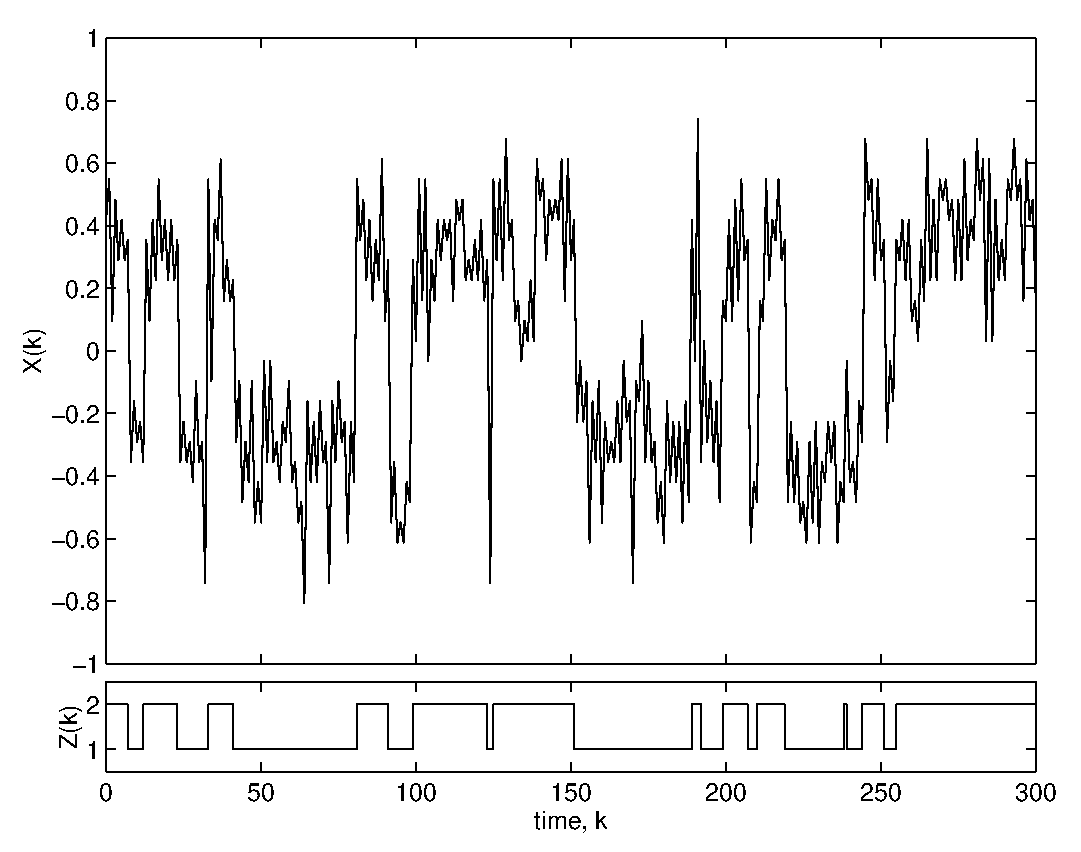
\includegraphics{fig/FigExTP1a_SamplePath.eps}}
  }
  \caption{\emph{The first 400 samples from a simulation of model A. The upper graph shows the turning points \emph{\texttt{x}} and the lower
    the regime process \emph{\texttt{z}}.}}
  \label{fig1:SamplePath}
\end{figure}


%%%%%%%%%%%%%%%%%%%%%%%%%%%%%%%%%%%%%%%%%%%%%%%
% Calculating the Rainflow Matrix
%%%%%%%%%%%%%%%%%%%%%%%%%%%%%%%%%%%%%%%%%%%%%%%

\subsection{Computing the Limiting Rainflow Matrix}

The two subloads are described by \verb+G1+ and \verb+G2+,
respectively, and their limiting rainflow matrices can be calculated
by the routine \verb+mctp2rfm+. The rainflow matrix for the
switching load is calculated by the routine \verb+smctp2rfm+ which
takes the transition matrix \verb+P+ together with \verb+G1+ and
\verb+G2+ as input.
\begin{code}
>> Grfc=smctp2rfm(P,{G1,[];G2,[]});
>> Grfc1=mctp2rfm({G1,[]});
>> Grfc2=mctp2rfm({G2,[]});
>> GrfcSum=statP(1)*Grfc1+statP(2)*Grfc2;
\end{code}
The matrix \verb+GrfcSum+ is a superposition of the rainflow
matrices for subloads 1 and 2, respectively. This is the rainflow
matrix we obtain if we don't take the switching into account. The
rainflow matrices can be plotted by \verb+cmatplot+.
\begin{code}
>> cmatplot(u,u,{Grfc1 Grfc2; GrfcSum Grfc})
\end{code}
%The calculated rainflow matrices for each regime \verb+Grfc1+,
%\verb+Grfc2+ and for the
%switching process \verb+Grfc+ are shown in
%Figure~\ref{fig1:rfc}a,b,c.
Note that, if
the  rainflow matrices for the two regimes are superimposed like
\verb+GrfcSum+, then the largest
cycles (low minima and large maxima) are lost, compare the two lower plots.
%Figure~\ref{fig1:rfc}c with~\ref{fig1:rfc}d.

%\begin{figure}[htbp]
%  \begin{tabular}{cc}
%    {\small (a) Rainflow matrix, \verb+Frfc1+}  &
%    {\small (b) Rainflow matrix, \verb+Frfc2+} \\
%    \resizebox{\figwidthB}{!}{\includegraphics{fig/Fig1rfc1.eps}} &
%    \resizebox{\figwidthB}{!}{\includegraphics{fig/Fig1rfc2.eps}} \\
%    {\small (c) Rainflow matrix, \verb+Frfc+}  &
%    {\small (d) Rainflow matrix, \verb+FrfcSum+} \\
%    \resizebox{\figwidthB}{!}{\includegraphics{fig/Fig1rfc.eps}} &
%    \resizebox{\figwidthB}{!}{\includegraphics{fig/Fig1rfcSum.eps}} \\
%  \end{tabular}
%  \caption{\emph{ 3D-plot of the rainflow
%      matrices
%      (a) regime 1,
%      (b) regime 2,
%      (c) switching process,
%      (d) weighted sum of regime 1 and 2.}}
%  \label{fig1:rfc}
%\end{figure}


%%%%%%%%%%%%%%%%%%%%%%%%%%%%%%%%%%%%%%%%%%%%%%%
% Model Definition and Simulation
%%%%%%%%%%%%%%%%%%%%%%%%%%%%%%%%%%%%%%%%%%%%%%%

\subsection{Model B (Optional)}

Skip this section if you don't have time, and come back to it later.

Here we shall examine model B in Table~\ref{TabMarkovTP:Templates}, the
same model as in \cite[p.~61, Example~4.2]{Johannesson99.PhD}. For
this model the subloads have the same mean level, equal to zero, but different
standard deviations.
The transition matrix \verb+P+ for the regime
process will be the same as before.
By using the routine \verb+mktestmat+, we specify the min-max
 matrices, \verb+G1B+ and \verb+G2B+.
\begin{code}
>> G1B = mktestmat(param,[-0.1 -0.1],0.28,0.5);  % regime 1
>> G2B = mktestmat(param,[0 0],0.12,2);          % regime 2
\end{code}
Plot the matrices \verb+G1B+ and \verb+G2B+ by using \verb+cmatplot+.
Simulate a load and plot it:
\begin{code}
>> [xDB,zB] = smctpsim(P,{G1B []; G2B []},T); % Simulate
>> xB=u(xDB)';                          % Change scale to levels -1,..,1
>> hmmplot(xB(t),zB(t),t,[1 2],'','',1) % Different colours
\end{code}
A simulated signal is shown in Figure~\ref{fig:SamplePathB}.

\begin{figure}[htbp]
  \centerline{
   \resizebox{\figwidthA}{\figheightA}{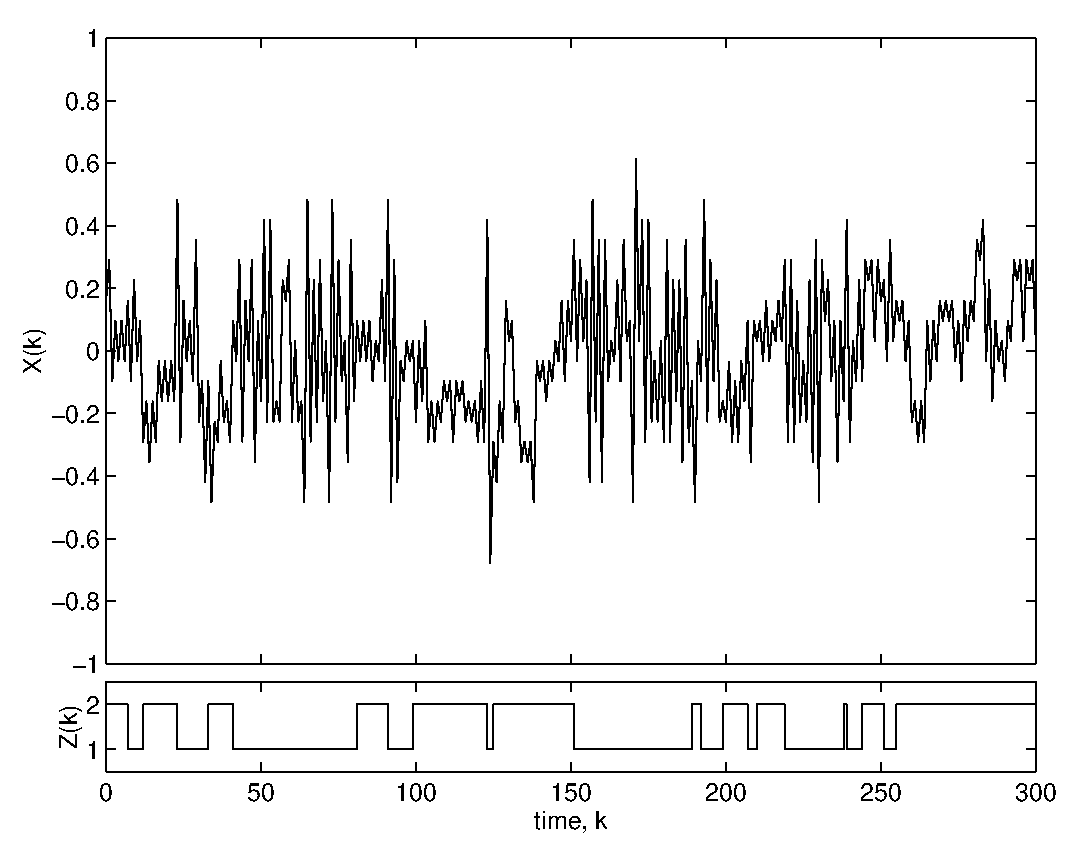
\includegraphics{fig/FigExTP1b_SamplePath.eps}}
  }
  \caption{\emph{The first 400 samples from a simulation of model B. The upper graph shows the turning points \emph{\texttt{x}} and the lower
    the regime process \emph{\texttt{z}}.}}
  \label{fig:SamplePathB}
\end{figure}

Next we calculate the rainflow matrices for the switching load, for
the subloads, and the superposition of the two subloads.
\begin{code}
>> GrfcB=smctp2rfm(P,{G1B,[];G2B,[]});
>> Grfc1B=mctp2rfm({G1B,[]});
>> Grfc2B=mctp2rfm({G2B,[]});
>> GrfcSumB=statP(1)*Grfc1B+statP(2)*Grfc2B;
\end{code}
Plot the matrices and compare \verb+GrfcB+ with \verb+GrfcSumB+.
What is your observations and conclusions?  Can you see the
switching when looking at the rainflow matrix?

%%%%%%%%%%%%%%%%%%%%%%%%%%%%%%%%%%%%%%%%%%%%%%%
% Observed Rainflow Matrix and Smoothing
%%%%%%%%%%%%%%%%%%%%%%%%%%%%%%%%%%%%%%%%%%%%%%%

\subsection{Observed Rainflow Matrix and Smoothing}

Now we consider model A again.
From the simulated load we can find the rainflow cycles and then
compute the observed rainflow matrix \verb+FrfcObs0+.
\begin{code}
>> TP = dat2tp([(1:T)' xD]);            % Turning points
>> RFC = tp2rfc(TP);                    % Rainflow cycles
>> paramD = [1 n n];
>> FrfcObs0 = cc2cmat(paramD,RFC);      % Observed rainflow matrix
\end{code}
For a discrete sequence of turning points (which \verb+xD+ is) one can
perform the above operation by one command
\begin{code}
>> FrfcObs = dtp2rfm(xD,n);             % Observed rainflow matrix
\end{code}
Compare the observed rainflow matrix \verb+FrfcObs+
%in Figure~\ref{fig1:rfcObs}a
with the theoretical one \verb+Grfc+.   %in Figure~\ref{fig1:rfc}c.
\begin{code}
>> cmatplot(u,u,{FrfcObs/(T/2) Grfc},1)
\end{code}

%\begin{figure}[htbp]
%  \centerline{
%  \begin{tabular}{cc}
%    {\small (a) Rainflow matrix, \texttt{FrfcObs}}   & {\small (b) Rainflow matrix, \texttt{FrfcSmooth}}  \\
%     \resizebox{\figwidthB}{!}{\includegraphics{fig/Fig1rfcObs.eps}} &
%    \resizebox{\figwidthB}{!}{\includegraphics{fig/Fig1rfcSmooth.eps}}
%  \end{tabular}
%  }
%  \caption{\emph{  (a) Observed rainflow matrix
%      \emph{\texttt{FrfcObs}} obtained from the simulation \emph{\texttt{x}}.
%      (b) \emph{\texttt{FrfcSmooth}} is obtained by smoothing \emph{\texttt{FrfcObs}}.  }}
%  \label{fig1:rfcObs}
%\end{figure}

If the observed rainflow matrix is too wiggly it can be smoothed
using \verb+smoothcmat+ to obtain a better estimate of the limiting
rainflow matrix. The smoothing procedure can also be used to
extrapolate (and interpolate) the observed rainflow matrix to cycles
that were not observed.
\begin{code}
>> h=0.8; FrfcSmooth = smoothcmat(FrfcObs,1,h);
>> cmatplot(u,u,{FrfcObs/(T/2) FrfcSmooth/(T/2) Grfc},1)
\end{code}
%Figure~\ref{fig1:rfcObs}b shows \verb+FrfcSmooth+ which has been
%obtained by smoothing \texttt{FrfcObs}.
The so called bandwidth
\verb+h+ is a smoothing parameter. Try different values of the
smoothing parameter \verb+h+ and see the difference.
A small \verb+h+ gives little smoothing, while a large \verb+h+ gives
much smoothing.

%%%%%%%%%%%%%%%%%%%%%%%%%%%%%%%%%%%%%%%%%%%%%%%
% Observed Rainflow Matrix and Smoothing
%%%%%%%%%%%%%%%%%%%%%%%%%%%%%%%%%%%%%%%%%%%%%%%

%\subsection{Extrapolation and Smoothing of Rainflow Matrices}
%
%To be added.

%%%%%%%%%%%%%%%%%%%%%%%%%%%%%%%%%%%%%%%%%%%%%%%
% Level Crossings
%%%%%%%%%%%%%%%%%%%%%%%%%%%%%%%%%%%%%%%%%%%%%%%

\subsection{Level Crossings}

Information about level crossings is contained in the rainflow
matrix.
\begin{code}
>> mu = cmat2lc(param,Grfc);
>> muSum = cmat2lc(param,GrfcSum);
>> muObs = cmat2lc(param,FrfcObs/(T/2));
>> subplot(2,1,1), plot(mu(:,1),mu(:,2),muSum(:,1),muSum(:,2),'--')
>> subplot(2,1,2), plot(mu(:,1),mu(:,2),muObs(:,1),muObs(:,2),'--')
\end{code}
%Figure~\ref{fig1:mu}a
The first plot compares the upcrossing intensity \verb+mu+ of
the switching load with the upcrossing intensity \verb+muSum+ of the
superimposed rainflow matrix.
Observe that, as expected, the switching gives rise
to more zero upcrossings than in the weighted sum of the individual
upcrossing intensities.
%In Fgure~\ref{fig1:mu}b
In the second plot the observed upcrossing intensity \verb+muObs+
is shown together with the theoretical one \verb+mu+.

%\begin{figure}[htbp]
%  \begin{tabular}{cc}
%    {\small (a) Crossing intensity} &
%    {\small (b) Crossing intensity} \\
%    \resizebox{\figwidthB}{!}{\includegraphics{fig/Fig1muSum.eps}} &
%    \resizebox{\figwidthB}{!}{\includegraphics{fig/Fig1muObs.eps}}
%  \end{tabular}
%  \caption{\emph{
%      (a) Level upcrossing intensity, \emph{\texttt{mu}} (--) compared
%      with the weighted sum \emph{\texttt{muSum}} (-- --).
%      (b) Level upcrossing intensity, \emph{\texttt{mu}} (--), compared with observed
%      upcrossing intensity \emph{\texttt{muObs}} (--) obtained from the
%      simulation \emph{\texttt{x}}.
%      }}
%  \label{fig1:mu}
%\end{figure}

%%%%%%%%%%%%%%%%%%%%%%%%%%%%%%%%%%%%%%%%%%%%%%%
% Damage
%%%%%%%%%%%%%%%%%%%%%%%%%%%%%%%%%%%%%%%%%%%%%%%

\subsection{Damage}

The toolbox contains routines for calculating the damage of a
load. The Palmgren-Miner damage hypothesis together with the W�hler
curve is used. This leads to the damage
\begin{equation}
  {\cal D}_{\beta} = \sum \frac{1}{N_{s_i}}
  = \sum K\left(S_i^{\rfc}\right)^{\beta}, \qquad
  S_i^{\rfc} = \left(M_i-m_i^{\rfc}\right)/2
\end{equation}
where $K$ and $\beta$ are material parameters. (The routines use
$K=1$.) The routines are  \verb+cc2dam+ for a cycle count (e.g.\
rainflow cycles) and
\verb+cmat2dam+ for a cycle matrix (e.g.\ rainflow matrix).
\begin{code}
>> beta = 4;
>> Dam = cmat2dam(param,Grfc,beta)
>> DamSum = cmat2dam(param,GrfcSum,beta)
>> DamObs = cc2dam(u(RFC),beta)/(T/2)
\end{code}
The calculated damages are scaled to damage per cycle, giving the results
\verb+Dam=0.0098+, \verb+DamSum=0.0017+ and for the simulation
\verb+DamObs=0.0097+. The damage from the simulation can also be
computed from \verb|FrfcObs| by using \verb|cmat2dam|.

The damage matrix is calculated by \verb+cmat2dmat+ and shows how the
damage is distributed among the different cycles. The sum of all the
elements in the damage matrix gives the total damage.
\begin{code}
>> Dmat = cmat2dmat(param,Grfc,beta);
>> DmatSum = cmat2dmat(param,GrfcSum,beta);
>> subplot(1,2,1), cmatplot(u,u,Dmat), axis('square'), v=axis;
>> subplot(1,2,2), cmatplot(u,u,DmatSum), axis('square'), axis(v)
\end{code}
Note that the rainflow matrix for the switching process gives much more
damage than that of the simple superposition.

%%%%%%%%%%%%%%%%%%%%%%%%%%%%%%%%%%%%%%%%%%%%%%%
% Decomposition of a Mixed rainflow matrix
%%%%%%%%%%%%%%%%%%%%%%%%%%%%%%%%%%%%%%%%%%%%%%%

\section{Decomposition of a Mixed Rainflow Matrix}
\label{lab2:Decomposition}

When collecting a load history, in the form of a rainflow matrix, all
the cycles of the switching load are stored in
one mixed rainflow matrix. Hence, there is a
need to interpret the mixed rainflow matrix, and e.g.\ tell how much
of the different load types a vehicle has experienced.

Here we will see that one can use the methods in \cite[Chapter~8]{Johannesson99.PhD} for decomposition of a mixed rainflow
matrix, i.e.\ methods for estimation of a SMCTP model given a
measurement of a mixed rainflow matrix.
Hence, the task is to estimate the
characteristics of the different subloads as well as the
characteristics of the switching between
the different subloads. The fact that we are able to
calculate the mixed expected rainflow matrix for a SMCTP model makes this estimation possible.
The principle of the decomposition is to find the best fit between the
measured rainflow matrix and the theoretically computed one, i.e.\ the
expected rainflow matrix. One problem is to decide what to mean by
``best fit''. The maximum likelihood (ML) method is often the best
method and yields the model that is ``the most probable one''. We will
propose an approximate ML estimator. There is also the
possibility to minimize the distance between the measured and the
theoretical rainflow matrices. We will propose three such distances,
namely the chi-square, the Hellinger, and the Kullback-Leibler distances.

\section{Model and Estimation}
\label{SecEst:ModelEstimation}

We want to estimate a SMCTP model, where the
number of regime states $r$ is fixed.
The model is parametrized by the min-max and the max-min transition
matrices
\begin{displaymath}
  \bm{Q}^{(1)},\ldots,\bm{Q}^{(r)}
  \qquad \mbox{and} \qquad
  \bmh{Q}^{(1)},\ldots,\bmh{Q}^{(r)}
\end{displaymath}
respectively,
and the transition matrix $\bm{P}$ for the regime process.

Obviously, one would like to estimate the whole model, i.e.\
%the number of subloads $r$,
the $\bm{P}$-matrix, and the subloads.
However, this is not possible, since the number of parameters in the
SMCTP model is larger than the number of observations, i.e.\ the
number of elements in the rainflow matrix.
Therefore, one
needs to impose some additional structure on the model in order to get fewer
parameters to estimate.

Sometimes the min-max matrices of the subprocesses
are known (or can be considered known) and thus the parameters of
the subloads are given.
Hence, in this case, only the transition matrix
$\bm{P}$ needs to be estimated.
For a SMCTP with two regime states we have a model with the parameters
\begin{displaymath}
  \bm{P}=\left(
    \begin{array}{cc}
      1-p_1 & p_1 \\
      p_2   & 1-p_2
    \end{array}
    \right),\quad
    \bm{Q}^{(1)},\bmh{Q}^{(1)},
    \bm{Q}^{(2)},\bmh{Q}^{(2)}
\end{displaymath}
and when the models of the subloads are known, then only the
parameters $\bm{\theta}=\left( p_1, p_2 \right)$ need to be estimated.
One such case is when the measured
rainflow matrix is believed to be a mixture of known standard
rainflow matrices, which could e.g.\ reflect different parts of a
testing track.
The goal is then to find the
proportion and the switching frequency of the different subprocesses.
All this information is contained in the $\bm{P}$ matrix.

Define a SMCTP model and simulate it in order to obtain an observed
mixed rainflow matrix.
\begin{code}
>> n = 8; param = [-1 1 n];
>> M1.x0=[-0.4 -0.3]; M1.s=0.15; M1.lam=1;
>> M2.x0=[0.3 0.4]; M2.s=0.15; M2.lam=1;
>> G1 = mktestmat(param,M1.x0,M1.s,M1.lam);
>> G2 = mktestmat(param,M2.x0,M2.s,M2.lam);
>> P=[1-0.1 0.1; 0.05 1-0.05]                % Transition matrix
>> [xD,z] = smctpsim(P,{G1 []; G2 []},5000); % Simulate
>> Fobs = dtp2rfm(xD,n);                     % observed mixed rainflow matrix
\end{code}
In order to get reasonably short computing times in Matlab when doing
the decomposition, we have chosen only 8 discrete levels.
However, the programs for doing the decomposition don't have any limitations in the size of the model.

\subsubsection*{Three Scenarios} \label{SecEst:Scenarios}

We will consider three cases of specifying the parameter vector $\bm{\theta}$, that we
want to estimate, depending on how much knowledge we have on the
min-max matrices. The approximate ML method will be used.
\begin{enumerate}
\item The min-max matrices of the subloads can be considered known, so
  that only the regime process is unknown, and only the parameters
  $p_1$ and $p_2$ need to be estimated.
  $\bm{\theta}=(p_1,~p_2)$
\begin{code}
>> known1.F = {G1 []; G2 []}; % known min-max and max-min matrices
>> init1.P = P;               % initial guess of P-matrix
>> [Fest1,Est1] = estsmctp(Fobs,'P','ML',known1,[],init1);
>> Est1.P                     % Estimated P-matrix
\end{code}
\item Here the  min-max matrix for each subload $z$ is
  specified, but we allow a translation $\tilde{m}_z$ and a scaling $\tilde{s}_z$,
  which are used
  as parameters for the subloads. The translation $\tilde{m}_z$ corresponds to a change of the mean
  level and the scaling $\tilde{s}_z$ corresponds to a change in the variance for the subload,
  i.e.\ a transformation of the form
  $X^{(z)}(t)=\tilde{s}_z \tilde{X}^{(z)}(t) + \tilde{m}_z$,
  where $\tilde{X}^{(z)}(t)$ is the process according to the specified
  min-max matrix.
  Now we have six parameters to estimate,\\
  $\bm{\theta}=(p_1,~p_2,~\tilde{m}_1,~\tilde{s}_1,~\tilde{m}_2,~\tilde{s}_2).$
\begin{code}
... Estimate ...
\end{code}
\item Here we will use, for each subload, the parametric model
  described by Eqs.~(8.15,8.16) with four
  parameters. In total this gives ten parameters to estimate,\\
  $\bm{\theta}=(p_1,~p_2,~x_{11}~,x_{21}~,s_1~,\lambda_1,~x_{12}~,x_{22}~,s_2~,\lambda_2)$.
\begin{code}
>> known3.Ffun = 'f_funm';   % Function for calculating a submodel
>> known3.trModel2X = 'tr_m2x'; % transform from Model to X-vector
>> known3.trX2Model = 'tr_x2m'; % transform from X-vector to model
>> known3.param =param;
>> init3.P = P;              % initial guess of P-matrix
>> init3.M = {M1 M2};        % initial guess of Models for min-max mat
>> [Fest3,Est3] = estsmctp(Fobs,'P,CalcF','ML',known3,[],init3);
>> Est3.P                    % Estimated P-matrix
>> Est3.M{:}                 % Estimated parameters in models
\end{code}
\end{enumerate}

\subsubsection*{Estimation from a Measurement of the Regime Process}

If the regime process $\{Z_k\}$ itself is observed, then one has as much
information about the switching that one can possibly get.
The ML estimates of $p_1$ and
$p_2$ can easily be obtained from the observed regime process,
$\bm{z}=\{z_k\}_{k=0}^T$, see \cite[Appendix~A]{Johannesson99.PhD}.
%This estimator
%will be denoted ML-z, and will serve as our reference
%estimator, as no other estimator can perform better than ML-z, by
%means of bias and variance. We will be happy if the performance of some other method
%is almost as good as ML-z.
\begin{code}
>> Pest_z = estmc(z,2)
\end{code}

Compare the estimated stationary distributions and the true one:
\begin{code}
>> mc2stat(Est1.P)
>> mc2stat(Est3.P)
>> mc2stat(Pest_z)
>> mc2stat(P)
\end{code}

\subsection*{Methods for Estimation (Optional)}

The four methods for estimation, described in
\cite[Section~8.2]{Johannesson99.PhD}, will now be examined. The first
method is the approximate maximum
likelihood (AML) estimator, where we assume that the sample of the
rainflow matrix is a sample from a multinomial distribution.
The next three methods are based on minimizing the
distance between the measured rainflow matrix and the expected
rainflow matrix. The distances that will be used are, the
chi-square distance ($\chi^2$), the Hellinger distance (HD), and the
Kullback-Leibler distance (KL).
The estimates are obtained by numerical optimization by using the
routine \verb+fmins+, see
\cite[Section~8.6]{Johannesson99.PhD} for further details.
\begin{code}
>> known.F = {G1 []; G2 []};   % known min-max and max-min matrices
>> init.P = P;                 % initial guess of P-matrix
>> [Fest,Est] = estsmctp(Fobs,'P','ML',known,[],init); Est.P
>> [Fest,Est] = estsmctp(Fobs,'P','chi2',known,[],init); Est.P
>> [Fest,Est] = estsmctp(Fobs,'P','HD',known,[],init); Est.P
>> [Fest,Est] = estsmctp(Fobs,'P','KL',known,[],init); Est.P
\end{code}

\renewcommand{\FileId}{File: lab3.tex, Last changed: 2005-04-14}

%%%%%%%%%%%%%%%%%%%%%%%%%%%%%%%%%%%%%%%%%%%%%%%
% Power Spectrum and Rainflow Analysis
%%%%%%%%%%%%%%%%%%%%%%%%%%%%%%%%%%%%%%%%%%%%%%%

%\cleardoublepage
\chapter{Power Spectrum and Rainflow Analysis}
\label{lab3}

In this exercise we present tools for computation of
rainflow matrices (and consequently fatigue failure predictors)
for Gaussian random loads. As was mentioned in Introduction,
a Gaussian load is uniquely defined by its mean value $m$ and
spectrum $S(\omega)$. For simplicity only, the mean is assumed to be
zero;  hence, the spectrum is the single input argument into the model.
The spectrum can be estimated from a measured record
(as we did in Computer Exercise 1) or theoretically derived,
as it is often the case  in fatigue damage analysis of sea vessels.

\section{Power Spectrum}

Choose any spectrum you wish to analyse. It can be an estimated
spectrum from Lab 1 or some standard spectra given in WAFO. Four
examples are given below:
\begin{code}
>> S=jonswap;
>> S=oscspec;
>> S=torsethaugen;
>> load deep.dat, S=dat2spec(deep);
\end{code}
Compute mean frequency $f_0$, standard deviation $\sigma$, and
irregularity factor $\alpha$ for the Gaussian process with computed
spectrum $S$. Solution:
\begin{code}
>> L=spec2mom(S,4);
>> f0=sqrt(L(2)/L(1))/2/pi
>> s=sqrt(L(1))
>> alfa=f0/(sqrt(L(3)/L(2))/2/pi)
\end{code}
The four spectra are unimodal and only the estimated spectrum can
be considered as a broad band spectrum.
For narrow band spectra, with one  mode, the
mean  frequency $f_0$ is close to the the mode of the spectrum.
Check it for your choice of spectrum.
\begin{code}
>> wspecplot(S);
>> 2*pi*f0
\end{code}



\textbf{ Remark.} The parameters $f_0$ and $\sigma$  are important
to perform a crude
analysis of the damage intensity of the load.
The mean frequency indicates a rate of
bigger cycles while $\sigma$ is the scaling factor for amplitudes.
The so-called moment method postulates that amplitudes of these cycles are
$\sigma\cdot R$, Rayleigh distributed (the pdf for a  Rayleigh variable is
$r\exp(-0.5r^2)$). This gives a very simple predictor of fatigue life time
$T^f$
$$
\hat T^f=\frac{1}{\gamma\,f_0E[(\sigma R)^\beta]}=
\frac{1}{\gamma\,f_0\sigma^\beta\,2^{\beta/2}\Gamma(\frac{\beta}{2}+1)}.
$$
As a matter of fact, one can prove that this predictor
is always conservative (gives
too short fatigue life than the one obtained by means of
rainflow method). Summarizing,
knowing $f_0$ and $\sigma$, the upper bound for the damage intensity can
be calculated. This is what the function \verb|spec2dplus| is computing.
If the spectrum is unimodal and particularly if it
is narrow banded, the method gives very accurate results.
Observe that in some special cases, when $\beta=1$ and as  $\beta$ goes to
infinity, the method is exact.
In addition,
this approach can be extended to non-Gaussian loads; then the crossing spectrum
$lc(u)$ has to be given. When the crossing spectrum $lc(u)$ is known,
one can compute conservative bounds for the
damage intensity by means of \verb|lc2dplus|. (Obviously for Gaussian loads,
 \verb|lc2dplus| gives the same results as \verb|spec2dplus|).

For the chosen spectrum, compute the conservative bound for the
predictor  of $T^f$, time to fatigue
failure. Use $\beta=3.0, 3.1, 3.2,\ldots, 5.0$ and
$\gamma=5\cdot10^{-9}$.
(Obviously, our examples are somewhat artificial since
the signals are not stresses and the parameters $\beta$ and $\gamma$
are not based on real tests.)
Computation of $\hat T^f$
\begin{code}
>> beta=3:0.1:5;
>> gam=5E-9;
>> dpl=gam*spec2dplus(S,beta);
>> Tfpl=(1./dpl)/3600/24  %in days
>> clf, plot(beta,Tfpl)
\end{code}


\section{Simulation of $X$ and the damage intensity}


In this section we shall simulate $X(t)$, extract rainflow cycles,
estimate damage intensity and derive an estimate of time to fatigue
failure $T^f$. If your spectrum is narrow banded, you should obtain
results close to the conservative bounds from the previous subsection.
For broad banded spectra the difference can be more relevant and
one may need to use other methods to derive estimates or $T^f$.

Suppose that one wishes to simulate $X(t)$ with approximatively
1000  non-negligible cycles. The duration time $T$ of the
signal is then $T=1000/f_0$. Compute (approximatively) the proportion
of fatigue lifetime consumed by $X(t)$, $0\le t\le T$,
in $\%$ ($100\%\,\,T/T^f$), for $\beta=4.22$ and $\gamma=5\cdot10^{-9}$.
Solution:
\begin{code}
>> T=1000/f0 % in seconds
>> gam=5E-9;
>> 100*T*gam*spec2dplus(S,4.22) % in percent
\end{code}


\textbf{Remark.} When one wishes to simulate the process $X(t)$ for
a given spectrum $S$, it may not be obvious how to choose an
appropriate sampling frequency. One possibility is to use the
highest angular frequency in the spectrum $\omega_{max}$, say. Then
a natural sampling frequency would be $f=\omega_{max}/2\pi$.
However, this is often a too low frequency to get correct values of
rainflow amplitudes. Simply, one would miss exact positions of local
maxima and minima in $X$, leading to  underestimation of rainflow
amplitudes. In many cases the choice of between 50 to 100 times
higher frequency than the mean frequency is giving good results. In
the following  example we will use ~$f=60f_0$, that gives 60000
observations for the chosen $T$ value.

We will simulate five sample paths of loads and compute the damage
intensity. The sampling interval is chosen to $dt=1/(60f_0)$. For
fast and accurate simulation, the spectrum is recomputed so that the
highest frequency $\omega_{max}=2\pi/dt$. Then $X(t)$ is simulated.
From the sample path, turning points are extracted and the rainflow
cycles are calculated. The damage intensity can then be computed,
and a prediction of the fatigue failure time $T^f$ obtained.
\begin{code}
>> max(S.w)/pi
>> dt=1./f0/60
>> S1=specinterp(S,dt);
>> [max(S1.w) pi/dt]
>> clf, wspecplot(S), hold on, wspecplot(S1,1,'r.')
>> clf, plot(beta,Tfpl)
>> hold on
>> for  i=1:5
>>   X=spec2sdat(S1,60000);
>>   tp=dat2tp(X);
>>   rfc=tp2rfc(tp);
>>   db=cc2dam(rfc,beta);
>>   plot(beta,(1000/f0)*(1./db)*(1/gam)/3600/24,'r.') % Tf in days
>> end
\end{code}


\section{Theoretical computation of damage intensity}

For more complicated spectra that are not unimodal, the moment method can be
too conservative. In order to illustrate this we choose the following spectrum
$$
S(\omega)=9\exp(-8(\omega-0.5)^2)
+2\exp(-2|w-2|^{1.4}).
$$
It can be created as follows
\begin{code}
>> S=createspec;
>> w=levels([0 4 253]);
>> S.S=2*exp(-2*abs(w-2).^1.4);
>> S.S=S.S+9*exp(-8*(w-0.5).^2);
>> S.w=w;
>> S.note=['S(w)=9*exp(-8(w-0.5)^2)+2*exp(-2|w-2|.^1.4)']
>> wspecplot(S)
\end{code}
Check the accuracy of the conservative bound for the damage intensity
by simulating 10 sample paths of the load.
\begin{code}
>> L=spec2mom(S,4);
>> f0=sqrt(L(2)/L(1))/2/pi
>> dpl=gam*spec2dplus(S,beta);
>> Tfpl=(1./dpl)/3600/24  %in days
>> dt=1./f0/60
>> S1=specinterp(S,dt);
>> figure(1)
>> clf, plot(beta,Tfpl)
>> hold on
>> for  i=1:10
>>   X=spec2sdat(S1,60000);
>>   tp=dat2tp(X);
>>   rfc=tp2rfc(tp);
>>   db=cc2dam(rfc,beta);
>>   plot(beta,(1000/f0)*(1./db)*(1/gam)/3600/24,'r.') % Tf in days
>> end
\end{code}
We turn now to alternative method of computation of the rainflow matrix
and damage intensity. The method consists of two steps. First, the
transition matrix from maximum to the following minimum
\verb|fMm|, say, in $X$, is computed using a generalized Rice's formula.
(Since numerical
integrations are needed, this step is relatively slow. The
accuracy parameter is called \verb|nit|$=0,\ldots,5$.
Higher \verb|nit| gives better approximation).
Next, the sequence of turning points is approximated by a MCTP. The methods
presented in Computer Exercise 2 then give the rainflow matrix.
\begin{code}
>> a=sqrt(L(3)/L(2))/2/pi
>> s=sqrt(L(1))
>> help spec2cmat
>> paramu=[-4.5*s 4.5*s 46];
>> nit=2;
>> figure(2), clf
>> [frfc fMm]=spec2cmat(S,[],'rfc',[],paramu,nit);
>> hold on, plot(rfc(:,2),rfc(:,1),'.')
>> clf, pdfplot(fMm)
>> dg=a*cmat2dam(paramu,frfc.f,beta);
>> figure(1), plot(beta,(1./dg)*(1/gam)/3600/24,'g') % Tf in days
\end{code}
For this broad banded spectrum the parameter \verb|nit|$=2$ is too low;
we propose to use \verb|nit|$=3$, but it can take 4 minutes to get
the results.
\begin{code}
>> figure(2), clf
>> [frfc1 fMm1]=spec2cmat(S,[],'rfc',[],paramu,3);
>> dg1=a*cmat2dam(paramu,frfc1.f,beta);
>> figure(1)
>> plot(beta,(1./dg1)*(1/gam)/3600/24,'k') % Tf in days
\end{code}
We turn now to some additional applications of the computed matrix
\verb|fMm|. (Those exercises are optional.)

First, the matrix can be used to simulate much longer and faster
sequences of turning points of $X$, than using \verb|spec2sdt|.
\begin{code}
>> help mctpsim
>> F{1,1}=fMm.f;
>> F{1,2}=fMm.f';
>> mctp=mctpsim(F,1000);
>> clf,plot(mctp(1:40))
\end{code}
Next, if the simulated sequence contains too many small amplitudes one can
derive the Markov matrix for the rainflow filtered sequence. It can be done as
follows: replace a few sub-diagonals in the \verb|frfc| matrix by zeros,
then invert  it to get the new transition matrix. Now you can
use it to simulate the filtered sequence of turning points.
\begin{code}
>> frfc1=zeros(size(frfc.f));
>> frfc1=triu(frfc.f,5);
>> fMm1=iter(frfc1,fMm.f,20,0.001);
>> clf,contour(fMm.f,20)
>> hold on,  contour(fMm1,20)
>> F{1,1}=fMm1;
>> F{1,2}=fMm1';
>> mctp1=mctpsim(F,1000);
>> clf, subplot(2,1,1)
>> plot(mctp(1:40))
>> subplot(2,1,2)
>> plot(mctp1(1:40))
\end{code}

\renewcommand{\FileId}{File: lab4.tex, Last changed: 2005-04-14}

%%%%%%%%%%%%%%%%%%%%%%%%%%%%%%%%%%%%%%%%%%%%%%%
% Analysis of Measured Loads
%%%%%%%%%%%%%%%%%%%%%%%%%%%%%%%%%%%%%%%%%%%%%%%

%\cleardoublepage
\chapter{Modelling of Measured Loads}

We want to model a measured load signal that changes characteristics
over time.
Suppose that a switching process would be an appropriate model for the
load.
Our strategy is then to fit a switching Markov chain of turning points
(SMCTP) to the measurements. This
model can then be used to calculate the expected rainflow matrix
for the load, or to simulate load processes.  The procedure is illustrated in the form of a flow chart in
Figure~\ref{FigFlowChart2}, which is explained and commented below.
\begin{figure}[htbp]
  % Figuren �r ritad i xfig och converteras med kommandot
  % fig2pstex fig/FigFlowChart2
  \begin{center}
    \resizebox{!}{!}{\input{fig/FigFlowChart2.pstex_t}}
  \end{center}
  \caption{\emph{Flow chart for the modelling of measurements of a load.}}
  \label{FigFlowChart2}
\end{figure}



%%%%%%%%%%%%%%%%%%%%%%%%%%%%%%%%%%%%%%%%%%%%%%%
% A Truck Load --- curves and straights
%%%%%%%%%%%%%%%%%%%%%%%%%%%%%%%%%%%%%%%%%%%%%%%

\section{Estimation from Time Signal}

In this example we have a measurement of a truck load, with the truck
driving on a road that consists of curves and straights with some
small bends, see~\cite[Example~6.3]{Johannesson99.PhD}.
The same piece of road has been measured twice.
The time signal is stored in the variable
\verb|x0| with time (seconds) in the first column and the load values
in the second column. Load and plot the data.
\begin{code}
>> load switchingload
>> plot(x0(:,1),x0(:,2))
\end{code}
The load changes
between two duty cycles which can be observed as changes in mean
and standard deviation.

%\begin{figure}[htbp]
%  \centerline{
%%    \resizebox{\figwidthA}{\figheightA}{\includegraphics{fig/FigExVolvoLV2_Load.eps}}
%  }
%  \caption{\emph{A measured truck load consisting of curves and straight
%      parts. Rainflow cycles with range smaller than the discretization step, $0.0429$, have been removed.}}
%  \label{FigEx3bVolvoLoad}
%\end{figure}

Does it seem appropriate to model the load
by a SMCTP model with two regime states?
%The load will be modelled %, following Figure~\ref{FigFlowChart2},
%by a time-reversible
%switching MCTP with two regime states.
The  two regime states represent straights
(regime 1, low
mean, large variation), and curves (regime 2, high mean, low variation).

First, we will remove small oscillations in the load, which
either come from measurement noise, or are irrelevant to the fatigue
damage. This is done by a rainflow filter, which deletes all rainflow cycles with ranges
smaller than a given threshold, which is often chosen as the
discretization step. Define the discretization and apply a rainflow filter:
\begin{code}
>> n = 32; param = [-1 1.2 n]; % Define discretization
>> u = levels(param);     % Discrete levels
>> delta = u(2)-u(1)      % Discretization step
>> TP = dat2tp(x0,delta); % Get turning points and rainflow filter
\end{code}
Compare the turning points of the original time signal with the
rainflow filtered turning points. How much does the rainflow filter
reduce the amount of data?
\begin{code}
>> TP0 = dat2tp(x0);
>> plot(x0(:,1),x0(:,2),TP0(:,1),TP0(:,2),TP(:,1),TP(:,2))
>> length(x0), length(TP0), length(TP)
\end{code}
Check the rainflow cycles and the damage before and after rainflow
filtering. Is there any significant difference? Try different values of
the damage exponent \verb|beta|.
\begin{code}
>> RFC0 = tp2rfc(TP0); subplot(1,2,1), ccplot(RFC0)
>> RFC = tp2rfc(TP);   subplot(1,2,2), ccplot(RFC)
>> beta = 6;                % Damage exponent
>> Dam0 = cc2dam(RFC0,beta) % Damage
>> Dam = cc2dam(RFC,beta)   % Damage, after rainflow filter
>> Dam/Dam0
\end{code}
%The rainflow filtering reduces the number of cycles by
%74 \%
%(from 1533 to 396), but less than $0.05~\%$ of the total damage was removed for
%$\beta>3$ ($10^{-3}~\%$ for $\beta=4$, and $10^{-6}~\%$ for
%$\beta=6$).

Examine the level crossing spectrum of the load by using \verb|tp2lc|, both for
the original sequence \verb|TP0| and for the rainflow filtered
sequence \verb|TP|.
Is there any difference between the two crossing spectra?
Is it possible, from the level crossings, to see that the load
consists of two subloads?

Examine if the load can be modelled as a Gaussian process by using
e.g.\ \verb|wnormplot|. Also compare the level crossing spectrum with
the one obtained from Rice's formula, see Computer
Exercise~\ref{lab1}.

Now we will discretize the load by using \verb|dat2dtp|, which makes
discretization to the nearest
discrete level.
\begin{code}
>> dtp = dat2dtp(param,TP,delta); % Discretized turning points
>> tp = [dtp(:,1) u(dtp(:,2))'];  % Discretized turning points
>> T = length(dtp);               % Number of turning points
>> clf, plot(x0(:,1),x0(:,2),TP(:,1),TP(:,2),tp(:,1),tp(:,2))
>> v=axis; hold on,
>> plot([v(1:2)],[u(2:end)'-delta/2 u(2:end)'-delta/2],'k:')
>> hold off, axis([v(1:2) param(1:2)])
\end{code}
What is the error
in damage due to the discretization?
\begin{code}
>> rfc = tp2rfc(tp);        % Get rainflow cycles
>> dam = cc2dam(rfc,beta)   % Damage, after discretization & rainflow filter
>> dam/Dam0
\end{code}
Next we will (by hand) identify the two duty cycles in the load
signal.
Find the times when load switches regime state, and split up the
load by using the routine \verb|splitload|. The first column of
\verb|tz| contains times (in seconds) and the second column contains the
regime state that the load switches to.
\begin{code}
>> tz = [2 2; 46.40 1; 114.5 2; 161 1; 225.1 2; 270 1; 337.5 2; ...
>> 384.8 1; 433.2 2; 600 1];
>> [xxd,xd,z] = splitload(dtp,tz);
>> plot(xxd{1}(:,1),xxd{1}(:,2))
>> plot(xxd{2}(:,1),xxd{2}(:,2))
>> hmmplot(xd(:,2),z,xd(:,1),[1 2],'','',1)
\end{code}
Here \verb|xxd{1}| and \verb|xxd{2}| contain subload 1 and 2,
respectively, \verb|xd| the switching load, and \verb|z| the regime
process.

%Then we identified the two duty cycles in the load signal,
% and calculated for each subload the
%min-max matrix and the max-min matrix.
%The discretization was made according to method 1 on
%page~\pageref{ChCycles:DiscMethod1}, discretization to the nearest
%discrete level, with $n=64$
%discretization levels, ranging from $u_1=-1.2$ to $u_n=1.5$.
%The min-max and max-min transition
%matrices were then obtained by using kernel
%smoothing and normalization.

\subsubsection*{Estimation of the Subloads}

%For simplicity we will
Now assume that the subloads are time-reversible, which
%from Section~\ref{SecMarkovTP:TimeReversibility}
implies that their expected
max-min matrices can be obtained from their respective expected min-max matrix through
$\bmh{G}=\bm{G}^T$.
For each subload we need to calculate the min-max and max-min
transition matrices
$\bm{Q}$ and $\bmh{Q}$, respectively. This can be done in the
following three steps:
\begin{enumerate}
\item \emph{Calculation of min-max matrix $\bm{F}$.} This is no
  problem if we have a measurement of  $\bm{F}$.
  (If instead we have measured the rainflow matrix $\bm{F}^{\rfc}$, it can be
  inverted to find the min-max matrix $\bm{F}$, see~\cite[Chapter~7]{Johannesson99.PhD}, and see also the routines
  \verb|rfm2mctp| and \verb|arfm2mctp|.)
  %Chapter~\ref{ChRainflowInversion}.
  In our case the subloads have been measured as time series and then it is
  straightforward to calculate the min-max matrix $\bm{F}$ (and
  max-min matrix $\bmh{F}$).
\begin{code}
>> dtp1 = dat2tp(xxd{1});
>> [mM1,Mm1] = tp2mm(dtp1);
>> F1 = dcc2cmat(mM1,n);
>> dtp2 = dat2tp(xxd{2});
>> [mM2,Mm2] = tp2mm(dtp2);
>> F2 = dcc2cmat(mM2,n);
>> cmatplot(u,u,{F1 F2})
\end{code}
\item \emph{Estimate $\bm{G}$ through smoothing.} To obtain an estimate of the expected min-max
 matrix $\bm{G}$, the min-max matrix $\bm{F}$ is
 smoothed using a 2-dimensional kernel smoother,
 see~\cite[Appendix~D]{Johannesson99.PhD}.
 %Appendix~\ref{AppKernel}.
\begin{code}
>> [G1s,h1] = smoothcmat(F1);
>> G1 = smoothcmat(F1,1,1.0,0);
>> [G2s,h2] = smoothcmat(F2);
>> G2 = smoothcmat(F2,1,0.8,0);
>> cmatplot(u,u,{G1s G2s; G1 G2})
>> cmatplot(u,u,{F1 F2; G1 G2})
\end{code}
Choose appropriate values of the smoothing parameter \verb|h|.
 (Here we can improve the estimates, if the max-min matrix
 $\bmh{F}$ is also used, by smoothing the sum
 $\bm{F}+\bmh{F}^T$, instead of smoothing only $\bm{F}$.)

\item \emph{Normalizing.} The min-max and max-min transition matrices
  $\bm{Q}$ and $\bmh{Q}$, respectively, are obtained from the expected min-max
  and max-min matrices $\bm{G}$ and
  $\bmh{G}=\bm{G}^T$, respectively, by normalizing each
  row sum to 1. This is done automatically by the programs
  (\verb|mctp2rfm| and \verb|smctp2rfm|).
\end{enumerate}


\subsubsection*{Estimation of the Regime Process}



The $\bm{P}$-matrix for the regime process is obtained through
ML-estimation
\begin{equation}
  \bm{P}^* = \left(
  \begin{array}{cc}
    1-p^*_{12} & p^*_{12} \\
    p^*_{21} & 1-p^*_{21}
  \end{array} \right)
\end{equation}
where
\begin{eqnarray}
  p^*_{12}
  &=& \frac{N_{12}}{N_1}=
  \frac{\#\{\mbox{Jumps from 1 to 2}\}}{N_1} =
  \frac{4}{N_1} = 0.0134, \\
  p^*_{21} &=& \frac{N_{21}}{N_2}=\frac{\#\{\mbox{Jumps from 2 to 1}\}}{N_2} =
  \frac{4}{N_2} = 0.0081 .
\end{eqnarray}
where $N_{ij}$ is the number of switches from regime state $i$ to
state $j$, and $N_i$
is the total number of turning points in regime state $i$.
Now we estimate \verb|P| from the rainflow filtered and discretized
load signal.
\begin{code}
>> N1 = length(dtp1), N2 = length(dtp2)
>> N12 = 4; N21 = 4;
>> p1=N12/N1; p2=N21/N2;
>> P = [1-p1 p1; p2 1-p2]  % P-matrix
>> statP = mc2stat(P)      % Stationary distribution
\end{code}

From the estimated SMCTP model (\verb|P|, \verb|G1|, and \verb|G2|), we can calculated the expected
rainflow matrix
%which is shown in Figures~\ref{FigEx3bRFCint}a,b.
\begin{code}
>> GG = {G1 []; G2 []};
>> [Grfc,mu_rfc] = smctp2rfm(P,GG);
>> cocc(param,RFC,Grfc)
>> Frfc = dtp2rfm(dtp(:,2),n);
>> cmatplot(u,u,{Frfc Grfc*T/2})
\end{code}
Calculate the damage and the damage matrix.
\begin{code}
>> beta = 6;
>> Dam0, Dam, dam
>> damG = cmat2dam(param,Grfc,beta)*T/2
>> damG/Dam0
>> beta = 4;
>> Dmat = cmat2dmat(param,Frfc,beta);
>> DmatG = cmat2dmat(param,Grfc,beta)*T/2;
>> cmatplot(u,u,{Dmat,DmatG},3)
\end{code}
Simulate the estimated SMCTP model and compare it with the measured signal.
\begin{code}
>> [xsim,zsim] = smctpsim(P,GG,T);
>> figure(1), hmmplot(u(xd(:,2))',z,1:length(xd),[1 2],'','',1)
>> figure(2), hmmplot(u(xsim)',zsim,1:T,[1 2],'','',1)
\end{code}
Make some more simulations and compare the simulated load signals.


%\begin{figure}[htbp]
%  \begin{tabular}{cc}
%    {\small (a) Rainflow matrix}  &
%    {\small (b) Rainflow matrix} \\
%    \resizebox{\figwidthB}{\figheightBB}{\includegraphics{fig/FigExVolvoLV2_RFMs.eps}} &
%    \resizebox{\figwidthB}{!}{\includegraphics{fig/FigExVolvoLV2_RFMsCC.eps}}\\
%    {\small (c) Crossing intensity, $\mu(u)$}  &
%    {\small (d) Damage} \\
%    \resizebox{\figwidthB}{!}{\includegraphics{fig/FigExVolvoLV2_Cross1.eps}} &
%     \resizebox{\figwidthB}{!}{\includegraphics{fig/FigExVolvoLV2_Dam.eps}}
%  \end{tabular}
%  \caption{\emph{Example~\ref{Ex3b}.
%      (a) 3D-plot of the expected rainflow matrix, $\bm{G}^{\rfc}$.
%      (b) Iso-lines of the expected rainflow matrix, $\bm{G}_T^{\rfc}$, together with rainflow cycles found in the load.
%      (c) Level upcrossing intensity, $\mu(u)$, compared with observed
%      upcrossing spectrum.
%      (d) Relative difference of damages,
%      $(\Dam_{\beta}(\bm{G}_T^{\rfc})-\Dam_{\beta}(X_k))/
%      \Dam_{\beta}(\bm{G}_T^{\rfc})$;
%      the mean \Solid,
%      the median \Dashdot,
%      the dashed lines \Dashed\ are the quantiles 0.1, 0.3, 0.7, 0.9,
%      obtained from 500 simulations of the estimated SMCTP model,
%      the \texttt{*}-line is the measured load, and
%      the $\Box$-line is the discretized measured load.
%      }}
%      \label{FigEx3bRFCint}
%\end{figure}


%%%%%%%%%%%%%%%%%%%%%%%%%%%%%%%%%%%%%%%%%%%%%%%
% A Truck Load --- curves and straights
%%%%%%%%%%%%%%%%%%%%%%%%%%%%%%%%%%%%%%%%%%%%%%%

\section{Decomposition of a Mixed Rainflow Matrix}



The goal of this example is to make a decomposition of the measured mixed
rainflow matrix, see~\cite[Example~8.1]{Johannesson99.PhD}.
The measurement is is the same  truck load as before.
We will make the decomposition with different assumptions on the
parametrization of the subloads, according to scenarios 1 and 3, see Section~\ref{lab2:Decomposition}.

In this example we will discretize the measured load by $n=16$ discrete
levels, ranging from $u_1=-1.0$ to $u_n=1.2$.
The pre-processing of the time signal is performed in the same way as previously.
\begin{code}
>> n = 16; param = [-1 1.2 n]; % Define discretization
>> u = levels(param);     % Discrete levels
>> delta = u(2)-u(1)      % Discretization step
>> TP = dat2tp(x0,delta); % Get turning points and rainflow filter
\end{code}
Check the difference in damage between the original load history and
the rainflow filtered one.

Next we will discretize the load and compute its damage.
\begin{code}
>> dtp = dat2dtp(param,TP,delta); % Discretized turning points
>> tp = [dtp(:,1) u(dtp(:,2))'];  % Discretized turning points
>> T = length(dtp);               % Number of turning points
>> rfc = tp2rfc(tp);        % Get rainflow cycles
>> beta = 6;
>> dam = cc2dam(rfc,beta)   % Damage, after discretization & rainflow filter
>> dam/Dam0
\end{code}
From the discretized load we compute the observed rainflow
matrix, which will be the input to the decomposition.
\begin{code}
>> Frfc = dtp2rfm(dtp(:,2),n);  % Observed rainflow matrix
\end{code}

For scenario 1, the min-max matrices \verb|G1| and \verb|G2| for the subloads
will be treated as a priori information, and will hence be considered
known. Therefore, for scenario 1, we only need to estimate the
$\bm{P}$-matrix with two parameters $p_1$ and $p_2$.
To obtain \verb|G1| and \verb|G2| we split the time signal,
and estimate them (and then forget about the time signal).
\begin{code}
>> tz = [2 2; 46.40 1; 114.5 2; 161 1; 225.1 2; 270 1; 337.5 2; ...
>> 384.8 1; 433.2 2; 600 1];
>> [xxd,xd,z] = splitload(dtp,tz);
>> hmmplot(xd(:,2),z,xd(:,1),[1 2],'','',1)
>> dtp1 = dat2tp(xxd{1});
>> [mM1,Mm1] = tp2mm(dtp1);
>> F1 = dcc2cmat(mM1,n);
>> G1 = smoothcmat(F1,1,1.0,0);
>> dtp2 = dat2tp(xxd{2});
>> [mM2,Mm2] = tp2mm(dtp2);
>> F2 = dcc2cmat(mM2,n);
>> G2 = smoothcmat(F2,1,0.8,0);
\end{code}
Plot the estimated matrices \verb|G1| and \verb|G2|.

By using the observed rainflow matrix \verb|Frfc| (and \verb|G1|
and \verb|G2|) we do the decomposition.
\begin{code}
>> known1.F = {G1 []; G2 []};   % known min-max and max-min matrices
>> init1.P = P;                 % initial guess of P-matrix
>> warning off                  % Don't display warnings
>> [Fest1,Est1] = estsmctp(Frfc,'P','ML',known1,[],init1);
>> Est1.P          % Estimated P-matrix
>> mc2stat(Est1.P) % Estimated stationary distribution
\end{code}

For scenario 3, we will for each subload use the simple parametric
model, which we used in Computer Exercise~\ref{lab2}.
Hence, for scenario 3, we have 10 parameters to estimate: $p_1$, $p_2$, and 4
parameters for each subload, \\
$\bm{\theta}=(p_1,~p_2,~x_{11}~,x_{21}~,s_1~,\lambda_1,~x_{12}~,x_{22}~,s_2~,\lambda_2)$.
\begin{code}
>> known3.Ffun = 'f_funm';      % Function for calculating a submodel
>> known3.trModel2X = 'tr_m2x'; % transform from Model to X-vector
>> known3.trX2Model = 'tr_x2m'; % transform from X-vector to model
>> known3.param = param;
>> init3.P = P;       % initial guess of P-matrix
>> M1.x0=[0.1 0.1]; M1.s=0.15; M1.lam=2; % submodel 1
>> M2.x0=[0.5 0.7]; M2.s=0.1; M2.lam=1;   % submodel 2
>> init3.M = {M1 M2}; % initial guess of Models for min-max matrices
\end{code}
To shorten the computation time you can lower the accuracy by setting the
input \verb|OPTIONS| which is used by \verb|fmins|. See help
\verb|options| for more details.
\begin{code}
>> OPTIONS(2)  = 1e-1;    % the termination tolerance for x;
>> OPTIONS(3)  = 1e-1;    % the termination tolerance for F(x);
>> [Fest3,Est3] = estsmctp(Frfc,'P,CalcF','ML',known3,[],init3);
>> Est3.P          % Estimated P-matrix
>> mc2stat(Est3.P) % Estimated stationary distribution
>> Est3.M{:}       % Estimated parameters in models
\end{code}

Compare the results (\verb|Fest1|, and \verb|Fest2|) in
terms of estimated $\bm{P}$-matrices and there
stationary distributions. Remember that the model estimated from the
time signal has transition
matrix \verb|P| and stationary distribution \verb|statP|.
Hopefully, you can observe that even though the estimates of the parameters $p_1$
and $p_2$
differs from \verb|P|, the estimates of the stationary
distribution are quite accurate.

For each estimated SMCTP model we can compute its expected damage
as a function of the damage exponent $\beta$.
We can also compute the damage from the measured time signal.
\begin{code}
>> beta = 3:0.2:8;
>> Dam0 = cmat2dam(param,Frfc,beta)/(T/2); % Damage from load signal
>> FrfcEst1 = smctp2rfm(Fest1.P,Fest1.F);
>> Dam1 = cmat2dam(param,FrfcEst1,beta);   % Damage, scenario 1
>> FrfcEst3 = smctp2rfm(Fest3.P,Fest3.F);
>> Dam3 = cmat2dam(param,FrfcEst3,beta);   % Damage, scenario 3
>> plot(beta,Dam0,'b',beta,Dam1,'r',beta,Dam3,'g')
>> plot(beta,Dam1./Dam0,'r',beta,Dam3./Dam0,'g')
\end{code}
Are the results, in terms of damage, acceptable?
Do they agree better for small or for large values of the damage exponent $\beta$.


%%%%%%%%%%%%%%%%%%%%%%%%%%%%%%%%%%%%%%%%%%%%%%%
% Appendix
%%%%%%%%%%%%%%%%%%%%%%%%%%%%%%%%%%%%%%%%%%%%%%%


%\part{Appendix}
\cleardoublepage
\appendix

\renewcommand{\chaptermark}[1]%
  {\markboth{\textsl{Appendix \thechapter. #1}}{}}

%\include{wafoAppX}


%%%%%%%%%%%%%%%%%%%%%%%%%%%%%%%%%%%%%%%%%%%%%%%
% Bibliography
%%%%%%%%%%%%%%%%%%%%%%%%%%%%%%%%%%%%%%%%%%%%%%%

\cleardoublepage

\renewcommand{\FileId}{\FileIdX}

%\addcontentsline{toc}{chapter}{Bibliography}

\bibliographystyle{abbrv}
%\nocite{Johannesson97.M1,Johannesson97.R2,Johannesson97.Lic,Johannesson98.A1,Johannesson98.C2}
%\nocite{Lindgren91.A1,Rychlik97.A1,Rychlik92.A2,Rychlik93.A1,
%  Ochi94.A1,
%  Krenk89.A1}
%\bibliography{/usr/matstat/pj/tex/inputs/ref}
\bibliography{lab}

\end{document}
